\chapter{Teoria}
\label{cap:teoria}

\section{Introducció}

Els nombres enters permeten comptar quantitats positives i negatives, expressar guanys i pèrdues, temperatures per sobre i per sota de zero, o desplaçaments en sentits oposats. Ara bé, en moltes situacions quotidianes els enters no són suficients.

Per exemple, si volem repartir \(3\) barres de pa entre \(6\) persones de manera que totes rebin la mateixa quantitat i no sobri res, no podem donar un nombre enter de barres a cada persona. Cal dividir la unitat en parts iguals. En aquest cas, cada persona rep mitja barra. De manera semblant, si repartim \(5\) litres d'aigua entre \(4\) recipients iguals, cada recipient rep una quantitat que no és un nombre enter de litres.

Aquestes situacions apareixen constantment: en repartiments, mesures, preus, descomptes, escales, proporcions, receptes, interessos bancaris o càlculs geomètrics. Per això necessitem nombres que expressin parts d'una unitat o quocients entre quantitats enteres.

La manera habitual de representar aquestes quantitats és mitjançant fraccions:
\[
\frac{1}{2},\qquad
\frac{5}{4},\qquad
\frac{15}{6}.
\]
Així, quan diem que \(3\) barres es reparteixen entre \(6\) persones, la quantitat que correspon a cadascuna es representa per
\[
\frac{3}{6}.
\]
Aquesta fracció representa el mateix nombre que
\[
\frac{1}{2},
\]
perquè repartir \(3\) barres entre \(6\) persones és equivalent a donar mitja barra a cadascuna.

La mateixa idea apareix en geometria. Si volem dividir un segment en parts iguals, o comparar dues longituds que no són múltiples enters l'una de l'altra, també necessitem expressar raons entre quantitats. Aquestes raons es poden representar amb fraccions i, més endavant, donen lloc a la proporcionalitat geomètrica.

Aquesta observació mostra una dificultat important: una mateixa quantitat pot tenir moltes representacions fraccionàries diferents. Per exemple,
\[
\frac{1}{2},\qquad
\frac{2}{4},\qquad
\frac{3}{6},\qquad
\frac{-1}{-2}
\]
representen el mateix nombre. Per tant, si volem construir rigorosament els nombres racionals, no n'hi ha prou amb introduir fraccions: cal identificar quines fraccions representen la mateixa quantitat.

En aquesta unitat construirem el conjunt dels nombres racionals a partir dels nombres enters. Ho farem definint una relació d'equivalència entre fraccions i considerant com a nombre racional cadascuna de les classes d'equivalència obtingudes. Després estudiarem les operacions, l'ordre, l'expressió decimal i diverses aplicacions dels nombres racionals.

\subsection{Interpretació geomètrica dels nombres racionals}
\label{subsec:interpretacio-geometrica-racionals}

La necessitat dels nombres racionals també apareix de manera natural en geometria. Si fixem un segment com a unitat, volem dividir-lo en parts iguals i considerar una d'aquestes parts, dues, tres, o més. Així, si un segment unitat es divideix en \(b\) parts iguals, cadascuna d'aquestes parts representa la fracció
\[
\frac{1}{b}.
\]
Si en prenem \(a\) parts, obtenim la quantitat representada per la fracció
\[
\frac{a}{b}.
\]

Aquesta interpretació permet entendre els nombres racionals com a punts sobre una recta numèrica. Fixem una recta orientada i un segment unitat que té com origen un punt \(0\) i com extrem un punt \(1\). Llavors, per representar el racional positiu \(\frac{a}{b}\), dividim el segment unitat en \(b\) parts iguals i prenem \(a\) d'aquestes parts en el sentit positiu de la recta.

\begin{figure}[h]
	\centering
	\begin{tikzpicture}[scale=1]
		\draw[->] (-0.5,0) -- (6.5,0);
		\foreach \x in {0,1,2,3,4,5,6}
		\draw (\x,0.08) -- (\x,-0.08);
		
		\node[above] at (0,0.3) {\(0\)};
		\node[above] at (5,0.3) {\(1\)};
		\node[below] at (0,-0.3) {\(O\)};
		\node[below] at (5,-0.3) {\(U\)};
		
		\foreach \x in {1,2,3,4}
		\draw[dashed] (\x,0.45) -- (\x,-0.45);
		
		\fill (3,0) circle (2pt);
		\node[above] at (3,0.5) {\(\frac{3}{5}\)};
		\node[below] at (3,-0.5) {\(P\)};
		
		\node at (2.5,0.8) {};
	\end{tikzpicture}
	\caption{Representació geomètrica del nombre racional \(\frac{3}{5}\).}
\end{figure}

En la figura anterior, el segment que va de \(0\) a \(1\) s'ha dividit en \(5\) parts iguals. El punt situat a \(3\) d'aquestes parts de l'origen representa el nombre racional \(\frac{3}{5}\).

Si el racional és negatiu, fem el mateix procés però en el sentit oposat. Així, el nombre
\[
-\frac{a}{b}
\]
es representa a l'esquerra de \(0\), a una distància de \(\frac{a}{b}\) unitats.

Aquesta construcció geomètrica mostra que una fracció no és només una expressió algebraica. També pot interpretar-se com una raó entre segments. Si \(P\) és el punt que representa \(\frac{a}{b}\), aleshores, en el cas positiu, podem escriure
\[
\frac{OP}{OU}=\frac{a}{b}.
\]

A més, la proporcionalitat de segments explica per què fraccions diferents poden representar el mateix punt de la recta. Per exemple,
\[
\frac{1}{2}
\qquad\text{i}\qquad
\frac{2}{4}
\]
representen el mateix punt, perquè dividir la unitat en \(2\) parts i prendre'n \(1\) dona la mateixa longitud que dividir-la en \(4\) parts i prendre'n \(2\).

\begin{figure}[h]
	\centering
	\begin{tikzpicture}[scale=1]
		\draw[->] (-0.5,0) -- (5.5,0);
		\foreach \x in {0,1,2,3,4,5}
		\draw (\x,0.08) -- (\x,-0.08);
		
		\node[below] at (0,0) {\(0\)};
		\node[below] at (4,0) {\(1\)};
		
		% divisió en 2 parts
		\draw[dashed] (2,0.55) -- (2,0.05);
		\node[left] at (0,0.5) {en \(2\) parts};
		
		% divisió en 4 parts
		\foreach \x in {1,2,3}
		\draw[dashed] (\x,-0.05) -- (\x,-0.55);
		\node[left] at (0,-0.7) {en \(4\) parts};
		
		\fill (2,0) circle (2pt);
		\node[above] at (2,0.55) {\(\frac{1}{2}\)};
		\node[below] at (2,-0.55) {\(\frac{2}{4}\)};
	\end{tikzpicture}
	\caption{Les fraccions \(\frac{1}{2}\) i \(\frac{2}{4}\) representen el mateix punt de la recta.}
\end{figure}

En general, les fraccions
\[
\frac{a}{b}
\qquad\text{i}\qquad
\frac{c}{d}
\]
representen la mateixa raó geomètrica si i només si
\[
ad=bc.
\]
Aquesta és exactament la condició que farem servir per definir la relació d'equivalència entre fraccions.

Així, la construcció dels nombres racionals té una doble arrel: d'una banda, respon a la necessitat algebraica de dividir enters; de l'altra, formalitza la idea geomètrica de raó entre segments i permet situar aquests nombres sobre la recta numèrica.

\section{Necessitat d'ampliar el conjunt dels nombres enters}

A la unitat anterior es va veure que els nombres enters amplien els nombres naturals perquè permeten resoldre equacions de la forma
\[
a+x=b
\]
sense exigir que \(b\) sigui més gran que \(a\). En efecte, en \(\Z\) sempre podem escriure
\[
x=b-a.
\]

Ara bé, els enters encara no són suficients per resoldre totes les equacions senzilles. Considerem una equació de la forma
\[
ax=b,
\qquad a,b\in\Z,\quad a\neq0.
\]
Aquesta equació no sempre té solució en \(\Z\). Per exemple,
\[
2x=1
\]
no té cap solució entera, perquè no existeix cap enter que multiplicat per \(2\) doni \(1\). Tanmateix, en els problemes de repartiment i mesura volem poder expressar aquesta solució: és el nombre que representa una meitat de la unitat.

En general, l'equació
\[
ax=b,
\qquad a\neq0,
\]
té solució en \(\Z\) si i només si \(a\) divideix \(b\). Si \(a\) no divideix \(b\), cal ampliar el conjunt dels nombres enters per poder representar el quocient de \(b\) entre \(a\).

Així, la necessitat d'introduir els nombres racionals apareix des de dues perspectives complementàries. D'una banda, des d'un punt de vista geomètric, volem representar sobre una recta punts que no corresponen a nombres enters, però que s'obtenen dividint la unitat en un nombre enter de parts iguals i prenent-ne un nombre enter de parts. Aquests punts expressen raons entre segments i permeten interpretar fraccions com \(\frac{1}{2}\), \(\frac{3}{5}\) o \(\frac{7}{4}\) com a posicions sobre la recta numèrica.

D'altra banda, des d'un punt de vista algebraic, volem ampliar el conjunt dels nombres enters per poder resoldre equacions de la forma
\[
ax=b,
\qquad a,b\in\Z,\quad a\neq0,
\]
també quan \(a\) no divideix \(b\). En aquest cas, la solució s'expressa mitjançant el quocient
\[
\frac{b}{a}.
\]

Per tant, els nombres racionals responen alhora a una necessitat geomètrica i a una necessitat algebraica: permeten representar raons de segments sobre la recta i, al mateix temps, fan possible la divisió entre enters sempre que el divisor sigui no nul.


\begin{exemple}
	Decidiu quines de les equacions següents tenen solució en \(\Z\):
	\[
	a)\quad 3x=12,
	\qquad
	b)\quad 4x=10,
	\qquad
	c)\quad -5x=20,
	\qquad
	d)\quad 6x=7.
	\]
\end{exemple}

\begin{solucio}
	L'equació \(3x=12\) té solució en \(\Z\), perquè \(3\) divideix \(12\). La solució és
	\[
	x=4.
	\]
	
	L'equació \(4x=10\) no té solució en \(\Z\), perquè \(4\) no divideix \(10\).
	
	L'equació \(-5x=20\) té solució en \(\Z\), perquè \(-5\) divideix \(20\). La solució és
	\[
	x=-4.
	\]
	
	Finalment, l'equació \(6x=7\) no té solució en \(\Z\), perquè \(6\) no divideix \(7\).
	
	Per tant, les equacions \(a)\) i \(c)\) tenen solució entera, mentre que \(b)\) i \(d)\) exigeixen ampliar el conjunt dels nombres enters.
\end{solucio}

\begin{exemple}
	Situeu sobre la recta numèrica els nombres racionals
	\[
	-\frac{2}{5},
	\qquad
	\frac{3}{4},
	\qquad
	\frac{7}{3}.
	\]
\end{exemple}

\begin{solucio}
	Fixem una recta orientada, amb el \(0\) a l'origen i el \(1\) a una unitat de distància cap a la dreta.
	
	Per situar
	\[
	-\frac{2}{5},
	\]
	dividim la unitat en \(5\) parts iguals i prenem \(2\) d'aquestes parts cap a l'esquerra de \(0\). Per tant, \(-\frac{2}{5}\) queda entre \(-1\) i \(0\).
	
	Per situar
	\[
	\frac{3}{4},
	\]
	dividim la unitat en \(4\) parts iguals i prenem \(3\) d'aquestes parts cap a la dreta de \(0\). Per tant, \(\frac{3}{4}\) queda entre \(0\) i \(1\).
	
	Finalment, per situar
	\[
	\frac{7}{3},
	\]
	apliquem la divisió euclidiana de \(7\) entre \(3\):
	\[
	7=3\cdot 2+1,
	\qquad 0\leq 1<3.
	\]
	Això vol dir que \(\frac{7}{3}\) queda després de \(2\) unitats completes i a una tercera part de la unitat següent. Per tant, per representar-lo sobre la recta, avancem primer fins al punt \(2\), dividim el segment que va de \(2\) a \(3\) en \(3\) parts iguals i prenem \(1\) d'aquestes parts.
	
	Així, el punt que representa \(\frac{7}{3}\) queda entre \(2\) i \(3\).
	
	\begin{center}
		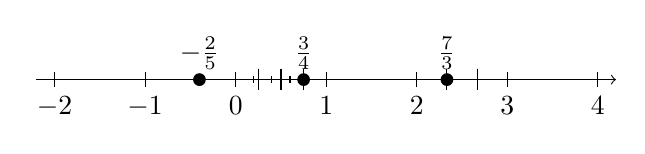
\begin{tikzpicture}[scale=1.15]
			
			% Recta
			\draw[->] (-2.2,0) -- (4.2,0);
			
			% Marques enteres
			\foreach \x/\lab in {-2/-2,-1/-1,0/0,1/1,2/2,3/3,4/4}
			{
				\draw (\x,0.08) -- (\x,-0.08);
				\node[below] at (\x,-0.08) {\(\lab\)};
			}
			
			% Punt -2/5
			\coordinate (A) at (-0.4,0);
			\fill (A) circle (2pt);
			\node[above] at (A) {\(-\frac{2}{5}\)};
			
			% Punt 3/4
			\coordinate (B) at (0.75,0);
			\fill (B) circle (2pt);
			\node[above] at (B) {\(\frac{3}{4}\)};
			
			% Punt 7/3
			\coordinate (C) at (2.333,0);
			\fill (C) circle (2pt);
			\node[above] at (C) {\(\frac{7}{3}\)};
			
			% Subdivisions entre 0 i 1 en cinquens
			\foreach \x in {0.2,0.4,0.6,0.8}
			\draw (\x,0.04) -- (\x,-0.04);
			
			% Subdivisions entre 0 i 1 en quarts
			\foreach \x in {0.25,0.5,0.75}
			\draw (\x,0.12) -- (\x,-0.12);
			
			% Subdivisions entre 2 i 3 en terços
			\foreach \x in {2.333,2.666}
			\draw (\x,0.12) -- (\x,-0.12);
			
		\end{tikzpicture}
		
		\smallskip
		\textit{Representació dels nombres racionals \(-\frac{2}{5}\), \(\frac{3}{4}\) i \(\frac{7}{3}\) sobre la recta numèrica.}
	\end{center}
	
	Aquest exemple mostra que els nombres racionals no només representen parts de la unitat situades entre \(0\) i \(1\). També poden ser negatius, com \(-\frac{2}{5}\), o més grans que \(1\), com \(\frac{7}{3}\). En tots els casos, però, es poden interpretar com a punts de la recta obtinguts a partir de divisions iguals de la unitat.
\end{solucio}

El pas de \(\Z\) a \(\Q\) és, doncs, anàleg al pas de \(\N\) a \(\Z\): ampliem el conjunt numèric per fer possible una operació que abans no sempre era possible. En passar de \(\N\) a \(\Z\), vam poder restar sense restriccions. En passar de \(\Z\) a \(\Q\), podrem dividir per qualsevol nombre no nul.

\section{Construcció del conjunt dels nombres racionals}

Intuïtivament, els nombres racionals són els punts de la recta que es poden obtenir dividint la unitat en un nombre enter de parts iguals i prenent-ne un nombre enter de parts. Equivalentment, són les quantitats que es poden expressar com una raó entre dos enters, amb denominador no nul. Així, la idea intuïtiva d'un nombre racional és la d'un quocient entre dos enters. Per representar aquest quocient escrivim una fracció
\[
\frac{a}{b},
\]
on
\[
a\in\Z,\qquad b\in\Z,\qquad b\neq0.
\]
El nombre \(a\) s'anomena \textbf{numerador} i el nombre \(b\) s'anomena \textbf{denominador}.

Escriurem
\[
\Zstar=\Z\setminus\{0\}.
\]
Així, formalment, una fracció es pot entendre com un parell ordenat
\[
(a,b)\in\Z\times\Zstar,
\]
que escrivim en la forma
\[
\frac{a}{b}.
\]
El denominador no pot ser zero, perquè la divisió per zero no està definida.

\begin{observacio}
	Com hem vist a la subsecció~\ref{subsec:interpretacio-geometrica-racionals},
	\emph{\nameref{subsec:interpretacio-geometrica-racionals}}, cal distingir entre fracció i nombre racional. Una fracció és una expressió de la forma \(\frac{a}{b}\), amb \(b\neq0\). Un nombre racional serà una classe de fraccions equivalents. Per tant, diferents fraccions poden representar el mateix nombre racional.
\end{observacio}

\subsection{Fraccions equivalents}

Dues fraccions
\[
\frac{a}{b}
\qquad\text{i}\qquad
\frac{c}{d},
\qquad b,d\neq0,
\]
són \textbf{equivalents} si compleixen
\[
ad=bc.
\]
En aquest cas escriurem
\[
\frac{a}{b}\sim\frac{c}{d}.
\]

Aquesta definició recull la idea habitual de fraccions que representen la mateixa quantitat. Per exemple, \(\frac{1}{2}\) i \(\frac{3}{6}\) representen la mateixa part de la unitat, i això queda reflectit en la igualtat
\[
1\cdot 6=2\cdot 3.
\]

\begin{exemple}
	Les fraccions \(\frac{2}{3}\) i \(\frac{8}{12}\) són equivalents, perquè
	\[
	2\cdot12=24
	\qquad\text{i}\qquad
	3\cdot8=24.
	\]
	Per tant,
	\[
	\frac{2}{3}\sim\frac{8}{12}.
	\]
\end{exemple}

\begin{exemple}
	Les fraccions \(\frac{-4}{5}\) i \(\frac{8}{-10}\) són equivalents, perquè
	\[
	(-4)\cdot(-10)=40
	\qquad\text{i}\qquad
	5\cdot8=40.
	\]
	Per tant,
	\[
	\frac{-4}{5}\sim\frac{8}{-10}.
	\]
\end{exemple}

\subsection{La relació d'equivalència}

La relació anterior permet agrupar totes les fraccions que representen la mateixa quantitat. Per poder fer-ho rigorosament, cal comprovar que és una relació d'equivalència.

\begin{proposicio}
	La relació \(\sim\) definida sobre \(\Z\times\Zstar\) per
	\[
	\frac{a}{b}\sim\frac{c}{d}
	\quad\Longleftrightarrow\quad
	ad=bc
	\]
	és una relació d'equivalència.
\end{proposicio}

\begin{prova}
	Cal comprovar que la relació és reflexiva, simètrica i transitiva.
	
	En primer lloc, és reflexiva. Per a qualsevol fracció \(\frac{a}{b}\), amb \(b\neq0\), tenim
	\[
	ab=ba.
	\]
	Per tant,
	\[
	\frac{a}{b}\sim\frac{a}{b}.
	\]
	
	En segon lloc, és simètrica. Suposem que
	\[
	\frac{a}{b}\sim\frac{c}{d}.
	\]
	Això vol dir que
	\[
	ad=bc.
	\]
	Per la commutativitat de la multiplicació en \(\Z\), aquesta igualtat equival a
	\[
	cb=da.
	\]
	Per tant,
	\[
	\frac{c}{d}\sim\frac{a}{b}.
	\]
	
	Finalment, és transitiva. Suposem que
	\[
	\frac{a}{b}\sim\frac{c}{d}
	\qquad\text{i}\qquad
	\frac{c}{d}\sim\frac{e}{f}.
	\]
	Això vol dir que
	\[
	ad=bc
	\qquad\text{i}\qquad
	cf=de.
	\]
	Multiplicant la primera igualtat per \(f\), obtenim
	\[
	adf=bcf.
	\]
	Com que \(cf=de\), podem substituir \(cf\) per \(de\):
	\[
	adf=bde.
	\]
	Com que \(d\neq0\), podem cancel·lar \(d\) i obtenim
	\[
	af=be.
	\]
	Per tant,
	\[
	\frac{a}{b}\sim\frac{e}{f}.
	\]
	Així, la relació és transitiva.
\end{prova}

\subsection{Definició del conjunt dels nombres racionals}

Com que \(\sim\) és una relació d'equivalència, podem considerar les seves classes d'equivalència.

La classe d'equivalència de la fracció \(\frac{a}{b}\) és el conjunt de totes les fraccions equivalents a \(\frac{a}{b}\):
\[
\left[\frac{a}{b}\right]
=
\left\{
\frac{x}{y}\in\Z\times\Zstar:
ay=bx
\right\}.
\]

\begin{definicio}
	El conjunt dels \textbf{nombres racionals} és el conjunt quocient
	\[
	\Q=(\Z\times\Zstar)/\sim.
	\]
	És a dir, un nombre racional és una classe d'equivalència de fraccions.
\end{definicio}

Així, el nombre racional representat per \(\frac{a}{b}\) és
\[
\left[\frac{a}{b}\right].
\]
Ara bé, per simplicitat, habitualment escriurem
\[
\frac{a}{b}
\]
per referir-nos al nombre racional representat per aquesta fracció. Aquest és un abús de notació habitual: identifiquem una fracció amb el nombre racional que representa.

\begin{exemple}
	Les fraccions
	\[
	\frac{1}{2},
	\qquad
	\frac{2}{4},
	\qquad
	\frac{3}{6},
	\qquad
	\frac{-1}{-2},
	\qquad
	\frac{-2}{-4}
	\]
	són equivalents i, per tant, representen el mateix nombre racional:
	\[
	\left[\frac{1}{2}\right]
	=
	\left[\frac{2}{4}\right]
	=
	\left[\frac{3}{6}\right]
	=
	\left[\frac{-1}{-2}\right].
	\]
	En la pràctica escrivim simplement
	\[
	\frac{1}{2}
	=
	\frac{2}{4}
	=
	\frac{3}{6}
	=
	\frac{-1}{-2}.
	\]
\end{exemple}

\subsection{Els enters com a nombres racionals}

Els nombres enters es poden veure de manera natural com a nombres racionals. Per fer-ho rigorosament, definim l'aplicació
\[
\iota:\Z\longrightarrow \Q
\]
donada per
\[
\iota(n)=\left[\frac{n}{1}\right].
\]
Aquesta aplicació està ben definida, perquè \(1\in\Zstar\), i per tant \(\frac{n}{1}\) és una fracció admissible per a tot \(n\in\Z\).

A més, \(\iota\) és injectiva. En efecte, si
\[
\iota(n)=\iota(m),
\]
aleshores
\[
\left[\frac{n}{1}\right]=\left[\frac{m}{1}\right].
\]
Per la definició de la relació d'equivalència entre fraccions, això vol dir que
\[
n\cdot 1=m\cdot 1,
\]
i, per tant,
\[
n=m.
\]
Així, dos enters diferents determinen dos nombres racionals diferents.

Per aquest motiu, podem identificar cada enter \(n\) amb el racional
\[
\left[\frac{n}{1}\right].
\]
Aquesta identificació permet considerar \(\Z\) com un subconjunt de \(\Q\), i escriure simplement
\[
\Z\subset \Q.
\]
A partir d'ara, quan no hi hagi risc de confusió, escriurem \(n\) en lloc de \(\left[\frac{n}{1}\right]\).

Aquesta inclusió és compatible amb les operacions, ja que
\[
\iota(n+m)=\iota(n)+\iota(m)
\]
i
\[
\iota(nm)=\iota(n)\iota(m).
\]


\subsection{Representants i fracció irreductible}

Com que un mateix nombre racional pot tenir molts representants, és útil escollir-ne un de especialment senzill.

Una fracció
\[
\frac{a}{b},
\qquad b>0,
\]
s'anomena \textbf{irreductible} si
\[
\mcd(a,b)=1.
\]
Això vol dir que el numerador i el denominador no tenen cap divisor comú positiu més gran que \(1\).

\begin{proposicio}
	Tot nombre racional es pot representar mitjançant una fracció irreductible amb denominador positiu.
\end{proposicio}

\begin{prova}
	Considerem una fracció qualsevol
	\[
	\frac{a}{b},
	\qquad b\neq0.
	\]
	Si \(b<0\), podem canviar el signe del numerador i del denominador:
	\[
	\frac{a}{b}
	=
	\frac{-a}{-b}.
	\]
	Així podem suposar que el denominador és positiu.
	
	Sigui
	\[
	g=\mcd(a,b).
	\]
	Aleshores podem escriure
	\[
	a=ga',
	\qquad
	b=gb',
	\]
	amb
	\[
	\mcd(a',b')=1.
	\]
	Per tant,
	\[
	\frac{a}{b}
	=
	\frac{ga'}{gb'}
	=
	\frac{a'}{b'}.
	\]
	La fracció \(\frac{a'}{b'}\) és irreductible i té denominador positiu.
\end{prova}

\begin{proposicio}
	La fracció irreductible amb denominador positiu que representa un nombre racional és única.
\end{proposicio}

\begin{prova}
	Suposem que
	\[
	\frac{a}{b}
	\qquad\text{i}\qquad
	\frac{c}{d}
	\]
	són dues fraccions irreductibles, amb
	\[
	b>0,\qquad d>0,
	\]
	i que representen el mateix nombre racional. Aleshores són equivalents i, per tant,
	\[
	ad=bc.
	\]
	
	Com que \(\mcd(a,b)=1\) i \(b\mid ad\), pel lema d'Euclides deduïm que
	\[
	b\mid d.
	\]
	De manera anàloga, com que \(\mcd(c,d)=1\) i \(d\mid bc\), deduïm que
	\[
	d\mid b.
	\]
	Per tant, \(b\) i \(d\) es divideixen mútuament. Com que tots dos són positius, obtenim
	\[
	b=d.
	\]
	Substituint en la igualtat \(ad=bc\), resulta
	\[
	ab=bc.
	\]
	Com que \(b\neq0\), podem cancel·lar \(b\), i obtenim
	\[
	a=c.
	\]
	Així, les dues fraccions són iguals.
\end{prova}

Per tant, cada nombre racional té un representant irreductible únic amb denominador positiu. Aquesta fracció és la forma més simple d'escriure el nombre racional.

\begin{exemple}
	Reduïm a fracció irreductible:
	\[
	\frac{180}{240}.
	\]
	Com que
	\[
	\mcd(180,240)=60,
	\]
	tenim
	\[
	\frac{180}{240}
	=
	\frac{180:60}{240:60}
	=
	\frac{3}{4}.
	\]
	Per tant, la fracció irreductible equivalent a \(\frac{180}{240}\) és
	\[
	\frac{3}{4}.
	\]
\end{exemple}

\begin{exemple}
	Escrivim amb denominador positiu i en forma irreductible:
	\[
	\frac{45}{-60}.
	\]
	Primer passem el signe negatiu al numerador:
	\[
	\frac{45}{-60}
	=
	-\frac{45}{60}.
	\]
	Com que
	\[
	\mcd(45,60)=15,
	\]
	obtenim
	\[
	-\frac{45}{60}
	=
	-\frac{3}{4}.
	\]
	Per tant,
	\[
	\frac{45}{-60}
	=
	-\frac{3}{4}.
	\]
\end{exemple}

\subsection{Simplificació i denominador comú}

Si multipliquem el numerador i el denominador d'una fracció pel mateix enter no nul, obtenim una fracció equivalent:
\[
\frac{a}{b}
=
\frac{ka}{kb},
\qquad k\in\Zstar.
\]
De la mateixa manera, si dividim el numerador i el denominador per un divisor comú, obtenim una fracció equivalent més simple. Aquest procés s'anomena \textbf{simplificació}.

També és habitual transformar diverses fraccions en fraccions equivalents amb un mateix denominador. Això serà útil per sumar, restar i comparar nombres racionals.

\begin{exemple}
	Simplifiqueu la fracció
	\[
	\frac{-84}{126}
	\]
	fins a obtenir-ne la fracció irreductible.
\end{exemple}

\begin{solucio}
	Per simplificar una fracció, calculem primer el màxim comú divisor del numerador i del denominador, prescindint del signe:
	\[
	\mcd(84,126)=42.
	\]
	Aleshores dividim numerador i denominador per \(42\):
	\[
	\frac{-84}{126}
	=
	\frac{-84:42}{126:42}
	=
	\frac{-2}{3}.
	\]
	Com que
	\[
	\mcd(2,3)=1,
	\]
	la fracció
	\[
	\frac{-2}{3}
	\]
	és irreductible.
	
	Per tant,
	\[
	\frac{-84}{126}=\frac{-2}{3}.
	\]
\end{solucio}

\begin{exemple}
	Transformem les fraccions
	\[
	\frac{14}{20},
	\qquad
	\frac{7}{15},
	\qquad
	\frac{5}{30}
	\]
	en fraccions equivalents amb el mateix denominador.
\end{exemple}

\begin{solucio}
	Calculem primer el mínim comú múltiple dels denominadors:
	\[
	20=2^2\cdot5,
	\qquad
	15=3\cdot5,
	\qquad
	30=2\cdot3\cdot5.
	\]
	Per tant,
	\[
	\mcm(20,15,30)=2^2\cdot3\cdot5=60.
	\]
	
	Ara hem de transformar cada fracció en una fracció equivalent amb denominador \(60\). Per fer-ho, mirem per quin factor cal multiplicar cada denominador. Aquest mateix factor s'ha de multiplicar també al numerador.
	
	Com que
	\[
	20\cdot3=60,
	\qquad
	15\cdot4=60,
	\qquad
	30\cdot2=60,
	\]
	obtenim
	\[
	\frac{14}{20}
	=
	\frac{14\cdot3}{20\cdot3}
	=
	\frac{42}{60},
	\]
	\[
	\frac{7}{15}
	=
	\frac{7\cdot4}{15\cdot4}
	=
	\frac{28}{60},
	\]
	i
	\[
	\frac{5}{30}
	=
	\frac{5\cdot2}{30\cdot2}
	=
	\frac{10}{60}.
	\]
	
	Així, les fraccions equivalents amb denominador comú són
	\[
	\frac{42}{60},
	\qquad
	\frac{28}{60},
	\qquad
	\frac{10}{60}.
	\]
\end{solucio}


\section{El cos dels nombres racionals}

Un cop construït el conjunt dels nombres racionals com el conjunt quocient
\[
	\Q=(\Z\times\Zstar)/\sim,
\]
cal definir-hi les operacions d'addició i de multiplicació.

Recordem que un nombre racional és una classe d'equivalència de fraccions. Per tant, quan escrivim
\[
	\left[\frac{a}{b}\right],
\]
no ens referim només a la fracció \(\frac{a}{b}\), sinó a tota la classe de fraccions equivalents a ella.

Això obliga a tenir una precaució fonamental: si definim una operació fent servir representants, hem de comprovar que el resultat no depèn dels representants triats. Aquesta és la idea de dir que una operació està ben definida.

\subsection{Addició de nombres racionals}

Siguin
\[
	x=\left[\frac{a}{b}\right],
	\qquad
	y=\left[\frac{c}{d}\right]
\]
dos nombres racionals, amb \(a,c\in\Z\) i \(b,d\in\Zstar\). Definim l'addició de \(x\) i \(y\) per
\[
	x+y
	=
	\left[\frac{a}{b}\right]
	+
	\left[\frac{c}{d}\right]
	=
	\left[\frac{ad+bc}{bd}\right].
\]
El nombre racional \(x+y\) s'anomena la suma de \(x\) i \(y\).

Aquesta expressió té sentit perquè \(b\neq0\) i \(d\neq0\), i per tant
\[
	bd\neq0.
\]
Com que l'operació està definida entre classes d'equivalència, cal comprovar que la definició no depèn del representant escollit. Per això provarem la proposició següent.

\begin{proposicio}
L'addició de nombres racionals està ben definida.
\end{proposicio}

\begin{prova}
Suposem que
\[
	\frac{a}{b}\sim\frac{a'}{b'}
	\qquad\text{i}\qquad
	\frac{c}{d}\sim\frac{c'}{d'}.
\]
Això vol dir que
\[
	ab'=a'b
	\qquad\text{i}\qquad
	cd'=c'd.
\]
Hem de veure que
\[
	\frac{ad+bc}{bd}
	\sim
	\frac{a'd'+b'c'}{b'd'}.
\]
Per la definició de fraccions equivalents, cal provar que
\[
	(ad+bc)b'd'=(a'd'+b'c')bd.
\]
Calculem el primer membre:
\[
	(ad+bc)b'd'
	=
	adb'd'+bcb'd'.
\]
Com que \(ab'=a'b\), tenim
\[
	adb'd'=a'bdd'.
\]
I com que \(cd'=c'd\), tenim
\[
	bcb'd'=bb'c'd.
\]
Per tant,
\[
	(ad+bc)b'd'
	=
	a'bdd'+bb'c'd.
\]
Ara bé,
\[
	(a'd'+b'c')bd
	=
	a'd'bd+b'c'bd
	=
	a'bdd'+bb'c'd.
\]
Els dos membres són iguals. Així,
\[
	\frac{ad+bc}{bd}
	\sim
	\frac{a'd'+b'c'}{b'd'}.
\]
Per tant, l'addició no depèn dels representants triats i està ben definida.
\end{prova}

Un cop sabem que l'addició està ben definida, podem usar la notació habitual
\[
	\frac{a}{b}+\frac{c}{d}
	=
	\frac{ad+bc}{bd},
\]
entenent que aquesta expressió és una manera abreujada d'escriure l'addició de les classes
\[
	\left[\frac{a}{b}\right]
	\quad\text{i}\quad
	\left[\frac{c}{d}\right].
\]

\begin{exemple}
Calculem
\[
	\left[\frac{2}{3}\right]
	+
	\left[\frac{5}{4}\right].
\]
Per la definició d'addició,
\[
	\left[\frac{2}{3}\right]
	+
	\left[\frac{5}{4}\right]
	=
	\left[\frac{2\cdot4+3\cdot5}{3\cdot4}\right]
	=
	\left[\frac{8+15}{12}\right]
	=
	\left[\frac{23}{12}\right].
\]
\end{exemple}

\subsection{Propietats de l'addició}

L'addició de nombres racionals té les mateixes propietats formals que l'addició d'enters.

\begin{proposicio}
Per a tots \(x,y,z\in\Q\), es compleixen les propietats següents:
\begin{enumerate}
	\item \textbf{Commutativitat de l'addició:}
	\[
		x+y=y+x.
	\]

	\item \textbf{Associativitat de l'addició:}
	\[
		(x+y)+z=x+(y+z).
	\]

	\item \textbf{Existència d'element neutre per a l'addició:}
	existeix un element \(0\in\Q\) tal que
	\[
		x+0=x.
	\]

	\item \textbf{Existència d'element oposat:}
	per a tot \(x\in\Q\), existeix un element \(-x\in\Q\) tal que
	\[
		x+(-x)=0.
	\]
\end{enumerate}
\end{proposicio}

\begin{prova}
Siguin
\[
	x=\left[\frac{a}{b}\right],
	\qquad
	y=\left[\frac{c}{d}\right],
	\qquad
	z=\left[\frac{e}{f}\right].
\]

La commutativitat es dedueix directament de la definició:
\[
	x+y
	=
	\left[\frac{ad+bc}{bd}\right],
\]
mentre que
\[
	y+x
	=
	\left[\frac{cb+da}{db}\right].
\]
Com que en \(\Z\) tenim
\[
	ad+bc=da+cb
	\qquad\text{i}\qquad
	bd=db,
\]
obtenim
\[
	x+y=y+x.
\]

L'associativitat es comprova de manera anàloga utilitzant l'associativitat i la distributivitat de l'addició i la multiplicació en \(\Z\).

L'element neutre de l'addició és
\[
	0=\left[\frac{0}{1}\right].
\]
En efecte,
\[
	\left[\frac{a}{b}\right]
	+
	\left[\frac{0}{1}\right]
	=
	\left[\frac{a\cdot1+b\cdot0}{b\cdot1}\right]
	=
	\left[\frac{a}{b}\right].
\]

Finalment, l'oposat de
\[
	x=\left[\frac{a}{b}\right]
\]
és
\[
	-x=\left[\frac{-a}{b}\right].
\]
En efecte,
\[
	\left[\frac{a}{b}\right]
	+
	\left[\frac{-a}{b}\right]
	=
	\left[\frac{ab+b(-a)}{b^2}\right]
	=
	\left[\frac{0}{b^2}\right]
	=
	\left[\frac{0}{1}\right].
\]
Per tant,
\[
	x+(-x)=0.
\]
\end{prova}

A partir de l'oposat, podem definir la resta de nombres racionals. Si \(x,y\in\Q\), definim
\[
	x-y=x+(-y).
\]

\subsection{Multiplicació de nombres racionals}

Siguin
\[
	x=\left[\frac{a}{b}\right],
	\qquad
	y=\left[\frac{c}{d}\right]
\]
dos nombres racionals, amb \(a,c\in\Z\) i \(b,d\in\Zstar\). Definim la multiplicació de \(x\) i \(y\) per
\[
	xy
	=
	\left[\frac{a}{b}\right]
	\cdot
	\left[\frac{c}{d}\right]
	=
	\left[\frac{ac}{bd}\right].
\]
El nombre racional \(xy\) s'anomena el producte de \(x\) i \(y\).

Aquesta expressió té sentit perquè \(bd\neq0\). Com que l'operació està definida entre classes d'equivalència, cal comprovar que la definició no depèn del representant escollit.

\begin{proposicio}
La multiplicació de nombres racionals està ben definida.
\end{proposicio}

\begin{prova}
Suposem que
\[
	\frac{a}{b}\sim\frac{a'}{b'}
	\qquad\text{i}\qquad
	\frac{c}{d}\sim\frac{c'}{d'}.
\]
Això vol dir que
\[
	ab'=a'b
	\qquad\text{i}\qquad
	cd'=c'd.
\]
Hem de veure que
\[
	\frac{ac}{bd}
	\sim
	\frac{a'c'}{b'd'}.
\]
Per la definició de fraccions equivalents, cal provar que
\[
	acb'd'=a'c'bd.
\]
Ara bé,
\[
	acb'd'
	=
	(ab')(cd').
\]
Com que
\[
	ab'=a'b
	\qquad\text{i}\qquad
	cd'=c'd,
\]
tenim
\[
	(ab')(cd')=(a'b)(c'd)=a'c'bd.
\]
Per tant,
\[
	acb'd'=a'c'bd.
\]
Així,
\[
	\frac{ac}{bd}
	\sim
	\frac{a'c'}{b'd'}.
\]
Per tant, la multiplicació no depèn dels representants triats i està ben definida.
\end{prova}

Un cop sabem que la multiplicació està ben definida, podem usar la notació habitual
\[
	\frac{a}{b}\cdot\frac{c}{d}
	=
	\frac{ac}{bd},
\]
entenent que aquesta expressió és una manera abreujada d'escriure la multiplicació de les classes
\[
	\left[\frac{a}{b}\right]
	\quad\text{i}\quad
	\left[\frac{c}{d}\right].
\]

\begin{exemple}
Calculem
\[
	\left[\frac{-3}{5}\right]
	\cdot
	\left[\frac{10}{9}\right].
\]
Per la definició de multiplicació,
\[
	\left[\frac{-3}{5}\right]
	\cdot
	\left[\frac{10}{9}\right]
	=
	\left[\frac{(-3)\cdot10}{5\cdot9}\right]
	=
	\left[\frac{-30}{45}\right]
	=
	\left[\frac{-2}{3}\right].
\]
\end{exemple}

\subsection{Propietats de la multiplicació}

\begin{proposicio}
Per a tots \(x,y,z\in\Q\), es compleixen les propietats següents:
\begin{enumerate}
	\item \textbf{Commutativitat de la multiplicació:}
	\[
		xy=yx.
	\]

	\item \textbf{Associativitat de la multiplicació:}
	\[
		(xy)z=x(yz).
	\]

	\item \textbf{Existència d'element neutre per a la multiplicació:}
	existeix un element \(1\in\Q\), diferent de \(0\), tal que
	\[
		x\cdot 1=x.
	\]

	\item \textbf{Existència d'invers multiplicatiu:}
	si \(x\neq0\), existeix un element \(x^{-1}\in\Q\) tal que
	\[
		xx^{-1}=1.
	\]
\end{enumerate}
\end{proposicio}

\begin{prova}
Siguin
\[
	x=\left[\frac{a}{b}\right],
	\qquad
	y=\left[\frac{c}{d}\right],
	\qquad
	z=\left[\frac{e}{f}\right].
\]

La commutativitat es dedueix de la commutativitat de la multiplicació en \(\Z\):
\[
	xy
	=
	\left[\frac{ac}{bd}\right],
	\qquad
	yx
	=
	\left[\frac{ca}{db}\right].
\]
Com que
\[
	ac=ca
	\qquad\text{i}\qquad
	bd=db,
\]
tenim
\[
	xy=yx.
\]

L'associativitat es comprova igualment a partir de l'associativitat de la multiplicació en \(\Z\).

L'element neutre de la multiplicació és
\[
	1=\left[\frac{1}{1}\right].
\]
En efecte,
\[
	\left[\frac{a}{b}\right]
	\cdot
	\left[\frac{1}{1}\right]
	=
	\left[\frac{a\cdot1}{b\cdot1}\right]
	=
	\left[\frac{a}{b}\right].
\]

Finalment, suposem que
\[
	x=\left[\frac{a}{b}\right]\neq0.
\]
Això equival a dir que \(a\neq0\), perquè
\[
	\left[\frac{a}{b}\right]
	=
	\left[\frac{0}{1}\right]
\]
si i només si
\[
	a\cdot1=0\cdot b,
\]
és a dir, si i només si \(a=0\).

Aleshores podem definir
\[
	x^{-1}
	=
	\left[\frac{b}{a}\right],
\]
ja que \(a\neq0\). Tenim
\[
	x\cdot x^{-1}
	=
	\left[\frac{a}{b}\right]
	\cdot
	\left[\frac{b}{a}\right]
	=
	\left[\frac{ab}{ba}\right]
	=
	\left[\frac{1}{1}\right].
\]
Per tant,
\[
	xx^{-1}=1.
\]
\end{prova}

\begin{definicio}
Siguin \(x,y\in\Q\), amb \(y\neq0\). Definim la divisió de \(x\) entre \(y\) per
\[
	\frac{x}{y}=x\cdot y^{-1}.
\]
És a dir, dividir per un nombre racional no nul és el mateix que multiplicar pel seu invers multiplicatiu.
\end{definicio}

Si
\[
	x=\left[\frac{a}{b}\right]
	\qquad\text{i}\qquad
	y=\left[\frac{c}{d}\right],
\]
amb \(a,c\in\Z\), \(b,d\in\Zstar\) i \(y\neq0\), aleshores \(c\neq0\). Per tant,
\[
	y^{-1}
	=
	\left[\frac{d}{c}\right].
\]
Així,
\[
	\frac{x}{y}
	=
	\left[\frac{a}{b}\right]
	\cdot
	\left[\frac{d}{c}\right]
	=
	\left[\frac{ad}{bc}\right].
\]

Un cop definida la divisió en \(\Q\), podem usar la notació habitual
\[
	\frac{\frac{a}{b}}{\frac{c}{d}}
	=
	\frac{ad}{bc},
	\qquad c\neq0,
\]
entenent que aquesta expressió és una manera abreujada d'escriure la divisió de les classes
\[
	\left[\frac{a}{b}\right]
	\quad\text{i}\quad
	\left[\frac{c}{d}\right].
\]

\begin{proposicio}[Distributivitat de la multiplicació respecte de l'addició]
Per a tots \(x,y,z\in\Q\), es compleix
\[
	x(y+z)=xy+xz.
\]
\end{proposicio}

\begin{prova}
Siguin
\[
	x=\left[\frac{a}{b}\right],
	\qquad
	y=\left[\frac{c}{d}\right],
	\qquad
	z=\left[\frac{e}{f}\right].
\]
Aleshores
\[
	y+z
	=
	\left[\frac{cf+de}{df}\right].
\]
Per tant,
\[
	x(y+z)
	=
	\left[\frac{a}{b}\right]
	\cdot
	\left[\frac{cf+de}{df}\right]
	=
	\left[\frac{a(cf+de)}{bdf}\right].
\]
D'altra banda,
\[
	xy
	=
	\left[\frac{ac}{bd}\right],
	\qquad
	xz
	=
	\left[\frac{ae}{bf}\right].
\]
Així,
\[
	xy+xz
	=
	\left[\frac{ac}{bd}\right]
	+
	\left[\frac{ae}{bf}\right]
	=
	\left[\frac{acbf+bdae}{b^2df}\right].
\]
Simplificant l'expressió del numerador,
\[
	acbf+bdae
	=
	ab(cf+de).
\]
Per tant,
\[
	xy+xz
	=
	\left[\frac{ab(cf+de)}{b^2df}\right].
\]
Aquesta fracció és equivalent a
\[
	\frac{a(cf+de)}{bdf},
\]
perquè s'ha obtingut multiplicant numerador i denominador per \(b\). Així,
\[
	xy+xz
	=
	\left[\frac{a(cf+de)}{bdf}\right].
\]
Per tant,
\[
	x(y+z)=xy+xz.
\]
\end{prova}

\subsection{\texorpdfstring{\ensuremath{\Q}}{Q} com a cos commutatiu}

Les propietats anteriors mostren que el conjunt dels nombres racionals, amb l'addició i la multiplicació que hem definit, té una estructura algebraica molt important.

\begin{proposicio}
El conjunt \(\Q\), amb les operacions d'addició i multiplicació definides anteriorment, és un cos commutatiu.
\end{proposicio}

\begin{prova}
Hem vist que l'addició en \(\Q\) és associativa i commutativa, té element neutre \(0\), i tot element té oposat.

També hem vist que la multiplicació en \(\Q\) és associativa i commutativa, té element neutre \(1\), i tot element no nul té invers multiplicatiu.

Finalment, la multiplicació és distributiva respecte de l'addició:
\[
	x(y+z)=xy+xz.
\]
Per tant, \(\Q\) és un cos commutatiu.
\end{prova}

\section{El cos ordenat dels nombres racionals}
\label{sec:cos-ordenat-racionals}

Un cop hem definit les operacions d'addició i multiplicació en \(\Q\), volem dotar aquest conjunt d'una relació d'ordre. Aquesta relació ha de ser coherent amb la interpretació geomètrica dels nombres racionals com a punts de la recta numèrica: si un nombre racional queda a l'esquerra d'un altre, direm que és menor.

Ara bé, com que els nombres racionals són classes d'equivalència de fraccions, cal definir l'ordre de manera que no depengui del representant escollit.

\subsection{Definició de l'ordre}

Recordem que tot nombre racional admet un representant amb denominador positiu. Per això, per definir l'ordre, prendrem sempre representants amb denominador positiu.

\begin{definicio}
Siguin \(x,y\in\Q\). Prenem representants
\[
	x=\left[\frac{a}{b}\right],
	\qquad
	y=\left[\frac{c}{d}\right],
\]
amb \(a,c\in\Z\) i \(b,d\in\N\setminus\{0\}\). Definim
\[
	x\leq y
\]
si, i només si,
\[
	ad\leq bc.
\]
\end{definicio}

És a dir,
\[
	\left[\frac{a}{b}\right]\leq
	\left[\frac{c}{d}\right]
	\qquad\Longleftrightarrow\qquad
	ad\leq bc,
\]
sempre que \(b>0\) i \(d>0\).

\begin{proposicio}
La relació d'ordre anterior està ben definida.
\end{proposicio}

\begin{prova}
Hem de comprovar que la definició no depèn dels representants triats.

Suposem que
\[
	\frac{a}{b}\sim\frac{a'}{b'}
	\qquad\text{i}\qquad
	\frac{c}{d}\sim\frac{c'}{d'},
\]
amb
\[
	b,d,b',d'>0.
\]
Això vol dir que
\[
	ab'=a'b
	\qquad\text{i}\qquad
	cd'=c'd.
\]

Suposem ara que
\[
	ad\leq bc.
\]
Com que \(b'd'>0\), podem multiplicar els dos membres de la desigualtat per \(b'd'\) i obtenim
\[
	adb'd'\leq bcb'd'.
\]
Ara bé,
\[
	adb'd'=(ab')dd'=a'bdd',
\]
i també
\[
	bcb'd'=bb'(cd')=bb'c'd.
\]
Per tant,
\[
	a'bdd'\leq bb'c'd.
\]
Com que \(bd>0\), podem cancel·lar aquest factor positiu i obtenim
\[
	a'd'\leq b'c'.
\]
Això prova que
\[
	\left[\frac{a'}{b'}\right]\leq
	\left[\frac{c'}{d'}\right].
\]

El raonament invers és anàleg. Per tant, la relació d'ordre no depèn dels representants escollits i està ben definida.
\end{prova}

Un cop sabem que l'ordre està ben definit, podem usar la notació habitual
\[
	\frac{a}{b}\leq\frac{c}{d}
	\qquad\Longleftrightarrow\qquad
	ad\leq bc,
\]
sempre que \(b>0\) i \(d>0\), entenent que aquesta expressió és una manera abreujada de comparar les classes
\[
	\left[\frac{a}{b}\right]
	\qquad\text{i}\qquad
	\left[\frac{c}{d}\right].
\]

\begin{observacio}
Si dues fraccions tenen el mateix denominador positiu, l'ordre es redueix a comparar els numeradors. En efecte, si \(b>0\), aleshores
\[
	\frac{a}{b}\leq\frac{c}{b}
	\qquad\Longleftrightarrow\qquad
	ab\leq bc
	\qquad\Longleftrightarrow\qquad
	a\leq c.
\]
\end{observacio}

\begin{exemple}
Compareu els nombres racionals
\[
	-\frac{2}{5}
	\qquad\text{i}\qquad
	\frac{1}{3}.
\]
\end{exemple}

\begin{solucio}
Els denominadors són positius. Per tant, comparem els productes creuats:
\[
	(-2)\cdot3=-6
	\qquad\text{i}\qquad
	5\cdot1=5.
\]
Com que
\[
	-6<5,
\]
tenim
\[
	-\frac{2}{5}<\frac{1}{3}.
\]
\end{solucio}

\subsection{Propietats de l'ordre}

\begin{proposicio}
La relació \(\leq\) definida en \(\Q\) és una relació d'ordre total. És a dir, per a tots \(x,y,z\in\Q\), es compleixen les propietats següents:
\begin{enumerate}
	\item \textbf{Reflexiva:}
	\[
		x\leq x.
	\]

	\item \textbf{Antisimètrica:}
	si \(x\leq y\) i \(y\leq x\), aleshores
	\[
		x=y.
	\]

	\item \textbf{Transitiva:}
	si \(x\leq y\) i \(y\leq z\), aleshores
	\[
		x\leq z.
	\]

	\item \textbf{Total:}
	per a tots \(x,y\in\Q\), es compleix
	\[
		x\leq y
		\qquad\text{o bé}\qquad
		y\leq x.
	\]
\end{enumerate}
\end{proposicio}

\begin{prova}
Siguin
\[
	x=\left[\frac{a}{b}\right],
	\qquad
	y=\left[\frac{c}{d}\right],
	\qquad
	z=\left[\frac{e}{f}\right],
\]
amb \(b,d,f>0\).

La propietat reflexiva és immediata, perquè
\[
	ab=ba,
\]
i per tant
\[
	\frac{a}{b}\leq\frac{a}{b}.
\]

Per provar l'antisimetria, suposem que
\[
	x\leq y
	\qquad\text{i}\qquad
	y\leq x.
\]
Això vol dir que
\[
	ad\leq bc
	\qquad\text{i}\qquad
	cb\leq da.
\]
Com que \(cb=bc\) i \(da=ad\), obtenim
\[
	ad=bc.
\]
Per tant,
\[
	\frac{a}{b}\sim\frac{c}{d},
\]
i així
\[
	x=y.
\]

Per provar la propietat transitiva, suposem que
\[
	x\leq y
	\qquad\text{i}\qquad
	y\leq z.
\]
Aleshores
\[
	ad\leq bc
	\qquad\text{i}\qquad
	cf\leq de.
\]
Multiplicant la primera desigualtat per \(f>0\), obtenim
\[
	adf\leq bcf.
\]
Multiplicant la segona desigualtat per \(b>0\), obtenim
\[
	bcf\leq bde.
\]
Per tant,
\[
	adf\leq bde.
\]
Com que \(d>0\), podem cancel·lar \(d\) i obtenim
\[
	af\leq be.
\]
Això vol dir que
\[
	x\leq z.
\]

Finalment, de l'ordre total en \(\Z\) es dedueix l'ordre total en \(\Q\). En efecte, donats \(x\) i \(y\), els enters \(ad\) i \(bc\) són comparables; per tant,
\[
	ad\leq bc
	\qquad\text{o bé}\qquad
	bc\leq ad.
\]
Això equival a dir que
\[
	x\leq y
	\qquad\text{o bé}\qquad
	y\leq x.
\]
\end{prova}

Definim també l'ordre estricte. Si \(x,y\in\Q\), escrivim
\[
	x<y
\]
si, i només si,
\[
	x\leq y
	\qquad\text{i}\qquad
	x\neq y.
\]
Equivalentment, si
\[
	x=\left[\frac{a}{b}\right],
	\qquad
	y=\left[\frac{c}{d}\right],
\]
amb \(b,d>0\), aleshores
\[
	x<y
	\qquad\Longleftrightarrow\qquad
	ad<bc.
\]

\subsection{Compatibilitat de l'ordre amb les operacions}

Perquè \(\Q\) sigui un cos ordenat, l'ordre ha de ser compatible amb l'addició i amb la multiplicació.

\begin{proposicio}
L'ordre de \(\Q\) és compatible amb l'addició. És a dir, si \(x,y,z\in\Q\) i
\[
	x\leq y,
\]
aleshores
\[
	x+z\leq y+z.
\]
\end{proposicio}

\begin{prova}
Siguin
\[
	x=\left[\frac{a}{b}\right],
	\qquad
	y=\left[\frac{c}{d}\right],
	\qquad
	z=\left[\frac{e}{f}\right],
\]
amb \(b,d,f>0\). Suposem que
\[
	x\leq y.
\]
Això vol dir que
\[
	ad\leq bc.
\]

Ara bé,
\[
	x+z
	=
	\left[\frac{af+be}{bf}\right],
\]
i
\[
	y+z
	=
	\left[\frac{cf+de}{df}\right].
\]
Per veure que \(x+z\leq y+z\), hem de comprovar que
\[
	(af+be)df\leq (cf+de)bf.
\]
Calculem:
\[
	(af+be)df
	=
	adf^2+bdef,
\]
i
\[
	(cf+de)bf
	=
	bcf^2+bdef.
\]
Com que \(ad\leq bc\) i \(f^2>0\), tenim
\[
	adf^2\leq bcf^2.
\]
Afegint \(bdef\) als dos membres, obtenim
\[
	adf^2+bdef\leq bcf^2+bdef.
\]
Per tant,
\[
	(af+be)df\leq (cf+de)bf,
\]
i així
\[
	x+z\leq y+z.
\]
\end{prova}

\begin{proposicio}
L'ordre de \(\Q\) és compatible amb la multiplicació per nombres racionals no negatius. És a dir, si \(x,y,z\in\Q\),
\[
	x\leq y
	\qquad\text{i}\qquad
	0\leq z,
\]
aleshores
\[
	xz\leq yz.
\]
\end{proposicio}

\begin{prova}
Siguin
\[
	x=\left[\frac{a}{b}\right],
	\qquad
	y=\left[\frac{c}{d}\right],
	\qquad
	z=\left[\frac{e}{f}\right],
\]
amb \(b,d,f>0\). Suposem que
\[
	x\leq y
	\qquad\text{i}\qquad
	0\leq z.
\]
Això vol dir que
\[
	ad\leq bc
\]
i, com que
\[
	0=\left[\frac{0}{1}\right],
\]
també vol dir que
\[
	0\cdot f\leq 1\cdot e,
\]
és a dir,
\[
	0\leq e.
\]

Ara bé,
\[
	xz
	=
	\left[\frac{ae}{bf}\right],
	\qquad
	yz
	=
	\left[\frac{ce}{df}\right].
\]
Per veure que \(xz\leq yz\), hem de comprovar que
\[
	ae\,df\leq ce\,bf.
\]
Aquesta desigualtat és equivalent a
\[
	adef\leq bcef.
\]
Com que \(ad\leq bc\), \(e\geq0\) i \(f>0\), podem multiplicar la desigualtat \(ad\leq bc\) per \(ef\geq0\), i obtenim
\[
	adef\leq bcef.
\]
Per tant,
\[
	xz\leq yz.
\]
\end{prova}

\begin{corollari}
Si \(x,y\in\Q\) i
\[
	0\leq x
	\qquad\text{i}\qquad
	0\leq y,
\]
aleshores
\[
	0\leq xy.
\]
\end{corollari}

\begin{prova}
Apliquem la proposició anterior a la desigualtat
\[
	0\leq x
\]
multiplicant per \(y\), que és no negatiu. Obtenim
\[
	0\cdot y\leq xy.
\]
Com que \(0\cdot y=0\), resulta
\[
	0\leq xy.
\]
\end{prova}

\begin{proposicio}
El conjunt \(\Q\), amb les operacions d'addició i multiplicació i amb l'ordre definit anteriorment, és un cos ordenat.
\end{proposicio}

\begin{prova}
Hem vist que \(\Q\), amb l'addició i la multiplicació, és un cos commutatiu. També hem vist que \(\leq\) és una relació d'ordre total en \(\Q\), compatible amb l'addició i amb la multiplicació per nombres no negatius.

Per tant, \(\Q\) és un cos ordenat.
\end{prova}

\subsection{Densitat dels nombres racionals}

Una de les propietats més importants de l'ordre dels nombres racionals és que entre dos nombres racionals diferents sempre hi ha un altre nombre racional.

\begin{proposicio}
El conjunt \(\Q\) és dens. És a dir, si \(x,y\in\Q\) i
\[
	x<y,
\]
aleshores existeix \(m\in\Q\) tal que
\[
	x<m<y.
\]
\end{proposicio}

\begin{prova}
Prenem
\[
	m=\frac{x+y}{2}.
\]
Com que \(x,y\in\Q\), també tenim \(m\in\Q\).

Com que
\[
	x<y,
\]
si afegim \(x\) als dos membres, obtenim
\[
	x+x<x+y.
\]
És a dir,
\[
	2x<x+y.
\]
Multiplicant per \(\frac{1}{2}>0\), resulta
\[
	x<\frac{x+y}{2}.
\]
Per tant,
\[
	x<m.
\]

De la mateixa manera, com que
\[
	x<y,
\]
si afegim \(y\) als dos membres, obtenim
\[
	x+y<y+y.
\]
És a dir,
\[
	x+y<2y.
\]
Multiplicant per \(\frac{1}{2}>0\), resulta
\[
	\frac{x+y}{2}<y.
\]
Per tant,
\[
	m<y.
\]
Així,
\[
	x<m<y.
\]
\end{prova}

\begin{exemple}
Trobeu un nombre racional situat estrictament entre
\[
	\frac{1}{3}
	\qquad\text{i}\qquad
	\frac{1}{2}.
\]
\end{exemple}

\begin{solucio}
Podem prendre la mitjana aritmètica:
\[
	m=
	\frac{\frac{1}{3}+\frac{1}{2}}{2}.
\]
Calculem:
\[
	\frac{1}{3}+\frac{1}{2}
	=
	\frac{2+3}{6}
	=
	\frac{5}{6}.
\]
Per tant,
\[
	m=
	\frac{\frac{5}{6}}{2}
	=
	\frac{5}{12}.
\]
Així,
\[
	\frac{1}{3}<\frac{5}{12}<\frac{1}{2}.
\]
\end{solucio}

\begin{observacio}
A més de ser dens, el conjunt dels nombres racionals té la propietat arquimediana. Això vol dir que, donat qualsevol nombre racional positiu \(x\), sempre podem trobar un nombre natural \(n\) prou gran perquè
\[
	n>x.
\]
Més generalment, si \(x,y\in\Q\) i \(x>0\), existeix un nombre natural \(n\) tal que
\[
	nx>y.
\]

Aquesta propietat expressa que els nombres naturals no queden acotats dins de \(\Q\): avançant prou vegades una mateixa quantitat racional positiva, podem superar qualsevol nombre racional donat.
\end{observacio}

\subsection{Valor absolut}

L'ordre també permet definir el valor absolut d'un nombre racional.

\begin{definicio}
Si \(x\in\Q\), definim el valor absolut de \(x\) per
\[
	|x|=
	\begin{cases}
		x, & \text{si } x\geq0,\\
		-x, & \text{si } x<0.
	\end{cases}
\]
\end{definicio}

Geomètricament, \(|x|\) representa la distància del punt \(x\) a l'origen de la recta numèrica.

\begin{exemple}
Tenim
\[
	\left|\frac{3}{5}\right|=\frac{3}{5},
	\qquad
	\left|-\frac{7}{4}\right|=\frac{7}{4},
	\qquad
	|0|=0.
\]
\end{exemple}

\begin{proposicio}
Per a tots \(x,y\in\Q\), es compleixen les propietats següents:
\begin{enumerate}
	\item \textbf{No-negativitat:}
	\[
		|x|\geq0.
	\]

	\item \textbf{Anul·lació:}
	\[
		|x|=0
		\qquad\Longleftrightarrow\qquad
		x=0.
	\]

	\item \textbf{Compatibilitat amb la multiplicació:}
	\[
		|xy|=|x|\,|y|.
	\]

	\item \textbf{Desigualtat triangular:}
	\[
		|x+y|\leq |x|+|y|.
	\]
\end{enumerate}
\end{proposicio}

\begin{prova}
La no-negativitat és conseqüència directa de la definició: si \(x\geq0\), aleshores \(|x|=x\geq0\); si \(x<0\), aleshores \(-x>0\), i per tant \(|x|=-x>0\).

També és clar que \(|x|=0\) si i només si \(x=0\).

La compatibilitat amb la multiplicació es comprova distingint els signes de \(x\) i \(y\). Si tenen el mateix signe, \(xy\geq0\), i si tenen signe contrari, \(xy<0\). En tots els casos s'obté
\[
	|xy|=|x|\,|y|.
\]

Finalment, per provar la desigualtat triangular, observem que sempre es compleix
\[
	-|x|\leq x\leq |x|
\]
i
\[
	-|y|\leq y\leq |y|.
\]
Sumant aquestes dues dobles desigualtats, obtenim
\[
	-\bigl(|x|+|y|\bigr)
	\leq
	x+y
	\leq
	|x|+|y|.
\]
Això implica
\[
	|x+y|\leq |x|+|y|.
\]
\end{prova}

\section{Expressió decimal dels nombres racionals}

Els nombres racionals també es poden expressar en forma decimal. Aquesta representació és molt útil en el càlcul pràctic, en les mesures, en els preus i en moltes aplicacions quotidianes.

Com que un nombre racional es pot representar per una fracció
\[
	\frac{a}{b},
	\qquad a\in\Z,\quad b\in\Zstar,
\]
la seva expressió decimal s'obté dividint \(a\) entre \(b\). Per simplificar l'estudi, suposarem habitualment que la fracció està escrita en forma irreductible i amb denominador positiu:
\[
	\frac{a}{b},
	\qquad b>0,\qquad \mcd(a,b)=1.
\]

\subsection{Decimals finits}

Alguns nombres racionals tenen una expressió decimal finita. Per exemple,
\[
	\frac{3}{4}=0{,}75,
	\qquad
	\frac{7}{10}=0{,}7,
	\qquad
	\frac{21}{8}=2{,}625.
\]

\begin{definicio}
Direm que un nombre racional té una expressió decimal finita si es pot escriure en la forma
\[
	\frac{m}{10^n},
\]
amb \(m\in\Z\) i \(n\in\N\).
\end{definicio}

Aquesta definició reflecteix el fet que els decimals finits són precisament els nombres que es poden escriure amb denominador una potència de \(10\).

\begin{proposicio}
Siguin \(a,b\in\Z\), amb \(b>0\), i suposem que
\[
	\mcd(a,b)=1.
\]
El nombre racional
\[
	\frac{a}{b}
\]
té una expressió decimal finita si, i només si, el denominador \(b\) és de la forma
\[
	b=2^r5^s
\]
per a certs \(r,s\in\N\).
\end{proposicio}

\begin{prova}
Suposem primer que
\[
	b=2^r5^s.
\]
Prenem un nombre natural \(n\) tal que
\[
	n\geq r
	\qquad\text{i}\qquad
	n\geq s.
\]
Aleshores
\[
	10^n=2^n5^n
\]
és múltiple de \(b\). Per tant, existeix un nombre natural \(k\) tal que
\[
	bk=10^n.
\]
Així,
\[
	\frac{a}{b}
	=
	\frac{ak}{bk}
	=
	\frac{ak}{10^n}.
\]
Per tant, \(\frac{a}{b}\) té una expressió decimal finita.

Recíprocament, suposem que \(\frac{a}{b}\) té una expressió decimal finita. Aleshores existeixen \(m\in\Z\) i \(n\in\N\) tals que
\[
	\frac{a}{b}=\frac{m}{10^n}.
\]
Això implica
\[
	a10^n=bm.
\]
Com que \(\mcd(a,b)=1\), el denominador \(b\) ha de dividir \(10^n\). Però
\[
	10^n=2^n5^n.
\]
Així, els únics factors primers que poden aparèixer en \(b\) són \(2\) i \(5\). Per tant,
\[
	b=2^r5^s
\]
per a certs \(r,s\in\N\).
\end{prova}

\begin{exemple}
Estudieu si el nombre racional
\[
	\frac{7}{40}
\]
té una expressió decimal finita.
\end{exemple}

\begin{solucio}
La fracció ja és irreductible i
\[
	40=2^3\cdot5.
\]
Per tant, el denominador només té com a factors primers el \(2\) i el \(5\). Així, \(\frac{7}{40}\) té una expressió decimal finita.

Per trobar-la, escrivim el denominador com una potència de \(10\). Com que
\[
	40\cdot25=1000,
\]
tenim
\[
	\frac{7}{40}
	=
	\frac{7\cdot25}{40\cdot25}
	=
	\frac{175}{1000}
	=
	0{,}175.
\]
\end{solucio}

\begin{exemple}
Estudieu si el nombre racional
\[
	\frac{5}{6}
\]
té una expressió decimal finita.
\end{exemple}

\begin{solucio}
La fracció \(\frac{5}{6}\) és irreductible i
\[
	6=2\cdot3.
\]
Com que el denominador té el factor primer \(3\), que no és ni \(2\) ni \(5\), el nombre racional \(\frac{5}{6}\) no té una expressió decimal finita.
\end{solucio}

\subsection{Decimals periòdics}

Quan una fracció irreductible no té una expressió decimal finita, la seva expressió decimal no acaba. Per exemple, en fer la divisió de \(1\) entre \(3\), obtenim
\[
	\frac{1}{3}=0{,}3333\ldots
\]
La xifra \(3\) es repeteix indefinidament. Per indicar aquesta repetició, en lloc d'escriure \(0{,}3333\ldots\), escriurem
\[
	0{,}\overline{3}.
\]
Així,
\[
	\frac{1}{3}=0{,}\overline{3}.
\]

De la mateixa manera,
\[
	\frac{2}{11}=0{,}181818\ldots=0{,}\overline{18},
\]
i
\[
	\frac{5}{6}=0{,}8333\ldots=0{,}8\overline{3}.
\]

\begin{definicio}
Un decimal periòdic és una expressió decimal en què, a partir d'una certa posició, es repeteix indefinidament un mateix bloc de xifres. Aquest bloc s'anomena període.
\end{definicio}

Si el període comença immediatament després de la coma decimal, diem que el decimal és periòdic pur. Per exemple,
\[
	0{,}\overline{27}=0{,}272727\ldots
\]
és periòdic pur.

Si abans del període hi ha algunes xifres que no es repeteixen, diem que el decimal és periòdic mixt. Per exemple,
\[
	1{,}4\overline{6}=1{,}46666\ldots
\]
és periòdic mixt.

\begin{proposicio}
Tot nombre racional té una expressió decimal finita o periòdica.
\end{proposicio}

\begin{prova}
Considerem un nombre racional representat per una fracció
\[
	\frac{a}{b},
	\qquad b>0.
\]
En fer la divisió de \(a\) entre \(b\), en cada pas apareix un residu. Per la divisió euclidiana, aquests residus només poden ser
\[
	0,1,2,\ldots,b-1.
\]
Per tant, només hi ha \(b\) residus possibles.

Si en algun moment apareix el residu \(0\), la divisió acaba i l'expressió decimal és finita.

Si el residu \(0\) no apareix, com que només hi ha un nombre finit de residus possibles, algun residu s'ha de repetir. A partir del moment en què un residu es repeteix, el procés de la divisió també es repeteix, i per tant les xifres decimals es repeteixen periòdicament.

Així, l'expressió decimal de qualsevol nombre racional és finita o periòdica.
\end{prova}

\begin{exemple}
Calculem l'expressió decimal de
\[
	\frac{5}{6}.
\]
\end{exemple}

\begin{solucio}
Fem la divisió:
\[
	5:6=0{,}8333\ldots
\]
El residu que es repeteix dona lloc a la repetició indefinida de la xifra \(3\). Per tant,
\[
	\frac{5}{6}=0{,}8\overline{3}.
\]
\end{solucio}

\subsection{Fracció generatriu d'un decimal finit}

Fins ara hem partit d'una fracció i n'hem estudiat l'expressió decimal. Ara farem el procés invers: partirem d'una expressió decimal i buscarem una fracció que la representi.

Aquesta fracció s'anomena \emph{fracció generatriu}, perquè és la fracció que genera aquell nombre decimal. És a dir, si en fem la divisió decimal, obtenim precisament l'expressió decimal donada.

En el cas dels decimals finits, trobar la fracció generatriu és senzill: només cal escriure el decimal amb denominador una potència de \(10\), segons el nombre de xifres decimals.

\begin{exemple}
Escriviu \(2{,}375\) com a fracció irreductible.
\end{exemple}

\begin{solucio}
Com que hi ha tres xifres decimals, escrivim
\[
	2{,}375=\frac{2375}{1000}.
\]
Ara simplifiquem:
\[
	\frac{2375}{1000}
	=
	\frac{95}{40}
	=
	\frac{19}{8}.
\]
Per tant,
\[
	2{,}375=\frac{19}{8}.
\]
\end{solucio}

\subsection{Fracció generatriu d'un decimal periòdic}

Els decimals periòdics també representen nombres racionals. Per trobar-ne la fracció generatriu, fem servir una equació.

\begin{exemple}
Escriviu
\[
	x=0{,}\overline{27}
\]
com a fracció.
\end{exemple}

\begin{solucio}
Com que el període té dues xifres, multipliquem per \(100\):
\[
	100x=27{,}\overline{27}.
\]
Restem les dues igualtats:
\[
	100x-x
	=
	27{,}\overline{27}-0{,}\overline{27}.
\]
Així,
\[
	99x=27.
\]
Per tant,
\[
	x=\frac{27}{99}=\frac{3}{11}.
\]
Així,
\[
	0{,}\overline{27}=\frac{3}{11}.
\]
\end{solucio}

\begin{exemple}
Escriviu
\[
	x=1{,}4\overline{6}
\]
com a fracció.
\end{exemple}

\begin{solucio}
En aquest cas hi ha una xifra no periòdica després de la coma i una xifra periòdica. Multipliquem primer per \(10\), per situar el període just després de la coma:
\[
	10x=14{,}\overline{6}.
\]
Ara multipliquem per \(10\) una altra vegada:
\[
	100x=146{,}\overline{6}.
\]
Restem:
\[
	100x-10x
	=
	146{,}\overline{6}-14{,}\overline{6}.
\]
Per tant,
\[
	90x=132.
\]
Així,
\[
	x=\frac{132}{90}=\frac{22}{15}.
\]
Per tant,
\[
	1{,}4\overline{6}=\frac{22}{15}.
\]
\end{solucio}

\begin{proposicio}
Un nombre és racional si, i només si, la seva expressió decimal és finita o periòdica.
\end{proposicio}

\begin{prova}
Hem vist que tot nombre racional té una expressió decimal finita o periòdica.

Recíprocament, si un nombre té una expressió decimal finita, es pot escriure amb denominador una potència de \(10\), i per tant és racional.

Si un nombre té una expressió decimal periòdica, el procediment anterior permet obtenir una equació en què desapareix la part periòdica. Això dona una fracció generatriu. Per tant, també és racional.

Així, els nombres racionals són exactament els nombres amb expressió decimal finita o periòdica.
\end{prova}

\section{Representació gràfica dels nombres racionals}

Recorda el \textbf{teorema de Tales}: els segments interceptats sobre dues
rectes $r$ i $r^{\prime}$ per un conjunt de paral·leles són proporcionals%
%original-height 4.4196cm;  cropleft "0";  croptop "1";  cropright "1";
\begin{center}
\includegraphics[
height=4.4899cm,
width=5.8386cm
]%
{img/rac2.jpg}%
\end{center}
\[
\frac{\overline{AB}}{\overline{A^{\prime}B^{\prime}}}=\frac{\overline{BC}%
}{\overline{B^{\prime}C^{\prime}}}=\frac{\overline{CD}}{\overline{C^{\prime
}D^{\prime}}}%
\]
Una de les aplicacions d’aquest teorema és la divisió d’un segment en
parts iguals: volem dividir el segment $\overline{AB}$ en cinc parts
iguals%
%original-height 1.296cm;  cropleft "0";  croptop "1";  cropright "1";
\begin{center}
\includegraphics[
height=1.3663cm,
width=5.3883cm
]%
{img/rac1.jpg}%
\end{center}
Per això tracem amb una regla una semirecta qualsevol amb origen en \(A\).
A partir d’aquest punt, mitjançant un compàs assenyalem cinc segments
iguals. Unim el punt \(M\) amb el punt \(B\). Ara mitjançant regla i escaire
tracem paral·leles a la recta que uneix $M$ i $B$ pels altres punts marcats.
El teorema de Tales assegura que els segments interceptats sobre el segment
\(AB\) són iguals.%
%original-height 4.7623cm;  cropleft "0";  croptop "1";  cropright "1";
\begin{center}
\includegraphics[
height=4.8326cm,
width=5.8386cm
]%
{img/rac3.jpg}%
\end{center}


\bigskip

Aquesta construcció geomètrica permetrà representar sobre una recta
tots els nombres racionals. En efecte, considerem una recta en què
s'han representat els nombres enters \(0\) i \(1\). Mitjançant la
construcció descrita anteriorment podem dividir la unitat, és a dir,
el segment determinat pels punts representats per \(0\) i \(1\), en cinc
parts iguals. Els punts així obtinguts es corresponen amb els
nombres racionals representats per les fraccions $1/5,2/5,3/5$ i $4/5$.%
%original-height 4{,}6041cm;  cropleft "0";  croptop "1";  cropright "1";
\begin{center}
\includegraphics[
height=4.6744cm,
width=8.591cm
]%
{img/rac4.jpg}%
\end{center}


Si ara volguéssim representar el nombre racional representat per la
fracció $18/5$, com en efectuar la divisió entera entre $18$ i $5$
s’obté%
\[
18=5\cdot3+3
\]
aleshores podem descompondre la fracció de la manera següent:%
\[
\frac{18}{5}=3+\frac{3}{5}%
\]
és a dir, hem separat la part entera de la fracció. Podem ara
representar el nombre racional considerat de la manera següent:%
%original-height 4{,}6041cm;  cropleft "0";  croptop "1";  cropright "1";
\begin{center}
\includegraphics[
height=4.6744cm,
width=8.591cm
]%
{img/rac5.jpg}%
\end{center}


En general, si volem representar un nombre racional positiu escrit com una fracció
\[
\frac{a}{b},
\qquad a,b\in\N,
\qquad b\neq0,
\]
podem aplicar la divisió euclidiana de \(a\) entre \(b\):
\[
a=bq+r,
\qquad 0\leq r<b.
\]
Aleshores
\[
\frac{a}{b}
=
\frac{bq+r}{b}
=
q+\frac{r}{b}.
\]
Això vol dir que el punt que representa \(\frac{a}{b}\) es troba entre els enters \(q\) i \(q+1\). Per ubicar-lo dins d'aquest segment unitat, dividim el segment en \(b\) parts iguals i en prenem \(r\). Si \(r=0\), el nombre racional coincideix amb l'enter \(q\).


\bigskip

Aquesta representació dels nombres racionals sobre una recta ajuda a
visualitzar-ne l'ordenació. Si col·loquem la unitat a la dreta del punt
origen \(0\), aleshores \(\alpha<\beta\) significa que el punt de la recta
corresponent al nombre racional \(\alpha\) es troba a l’esquerra del
punt corresponent a \(\beta\).

\begin{exemple}
Representeu el nombre racional representat per la fracció \(-31/6\)
com un punt d’una recta.
\end{exemple}

\begin{solucio}
Com que
\[
-31=6\cdot(-6)+5
\]
aleshores podem descompondre la fracció de la manera següent:%
\[
-\frac{31}{6}=-6+\frac{5}{6}%
\]
Per tant, el punt es trobarà en el segment unitat determinat pels
enters \(-6\) i \(-5\). Dividint aquest segment en sis parts iguals i
prenent-ne després cinc obtenim el punt que representa el nombre
racional considerat.%
%original-height 5.0808cm;  cropleft "0";  croptop "1";  cropright "1";
\begin{center}
\includegraphics[
height=5.1511cm,
width=9.2258cm
]%
{img/rac6.jpg}%
\end{center}

\end{solucio}

\section{Potències de nombres racionals}

De manera anàloga a com definim les potències de nombres enters,
definirem ara les potències de base un nombre racional i exponent
natural. Escrivim abreujadament la multiplicació repetida de fraccions iguals%
\[
\overset{n\text{ vegades}}{\overbrace{\frac{a}{b}\cdot\cdots\cdot\frac{a}{b}}}%
\]
com%
\[
\left(  \frac{a}{b}\right)  ^{n}%
\]
que es defineix com la \textbf{potència} de \textbf{base} el nombre
racional representat per la fracció \(a/b\) i \textbf{exponent} natural
\(n\), o simplement, potència \(n\)-ésima del nombre racional
representat per \(a/b\). Per exemple,%
\[
\frac{2}{3}\cdot\frac{2}{3}\cdot\frac{2}{3}=\left(  \frac{2}{3}\right)  ^{3}%
\]


Evidentment, com%
\[
\overset{n\text{ vegades}}{\overbrace{\frac{a}{b}\cdot\cdots\cdot\frac{a}{b}}%
}=\frac{\overset{n\text{ vegades}}{\overbrace{a\cdot\cdots\cdot a}}%
}{\overset{n\text{ vegades}}{\overbrace{b\cdot\cdots\cdot b}}}=\frac{a^{n}%
}{b^{n}}%
\]
deduïm que%
\[
\left(  \frac{a}{b}\right)  ^{n}=\frac{a^{n}}{b^{n}}%
\]
Per tant, per elevar una fracció a un nombre natural s’eleva
numerador i denominador a aquest nombre.

\subsection{Propietats de les potències}

Les potències de nombres racionals satisfan les mateixes propietats formals que les potències de nombres enters, sempre que les expressions que apareixen tinguin sentit. En particular, cal tenir cura quan la base és \(0\) i apareixen exponents negatius.

\begin{proposicio}
Siguin \(x,y\in\Q\) i siguin \(m,n\in\N\). Es compleixen les propietats següents:
\begin{enumerate}
	\item \textbf{Producte de potències de la mateixa base:}
	\[
		x^m\cdot x^n=x^{m+n}.
	\]

	\item \textbf{Quocient de potències de la mateixa base:}
	si \(x\neq0\) i \(m\geq n\), aleshores
	\[
		\frac{x^m}{x^n}=x^{m-n}.
	\]

	\item \textbf{Potència d'una potència:}
	\[
		\left(x^m\right)^n=x^{mn}.
	\]

	\item \textbf{Potència d'un producte:}
	\[
		(xy)^n=x^n y^n.
	\]

	\item \textbf{Potència d'un quocient:}
	si \(y\neq0\), aleshores
	\[
		\left(\frac{x}{y}\right)^n=\frac{x^n}{y^n}.
	\]
\end{enumerate}
\end{proposicio}

\begin{prova}
La primera propietat es dedueix directament de la definició de potència. En efecte, \(x^m\) és el producte de \(m\) factors iguals a \(x\), i \(x^n\) és el producte de \(n\) factors iguals a \(x\). Per tant, el producte
\[
	x^m\cdot x^n
\]
conté en total \(m+n\) factors iguals a \(x\), i això és precisament
\[
	x^{m+n}.
\]

La propietat del quocient es dedueix de la propietat anterior i de l'existència d'invers multiplicatiu per als nombres racionals no nuls. Si \(x\neq0\) i \(m\geq n\), podem escriure
\[
	x^m=x^{m-n+n}=x^{m-n}\cdot x^n.
\]
Per tant,
\[
	\frac{x^m}{x^n}
	=
	\frac{x^{m-n}\cdot x^n}{x^n}
	=
	x^{m-n}.
\]

La propietat de la potència d'una potència també es dedueix de la definició: l'expressió
\[
	\left(x^m\right)^n
\]
és el producte de \(n\) factors iguals a \(x^m\). Com que cadascun d'aquests factors conté \(m\) factors iguals a \(x\), el resultat conté \(mn\) factors iguals a \(x\). Per tant,
\[
	\left(x^m\right)^n=x^{mn}.
\]

La propietat de la potència d'un producte es dedueix de l'associativitat i la commutativitat de la multiplicació en \(\Q\):
\[
	(xy)^n
	=
	\underbrace{(xy)(xy)\cdots(xy)}_{n\text{ factors}}
	=
	\underbrace{x x\cdots x}_{n\text{ factors}}
	\underbrace{y y\cdots y}_{n\text{ factors}}
	=
	x^n y^n.
\]

Finalment, si \(y\neq0\), tenim
\[
	\frac{x}{y}=xy^{-1}.
\]
Aleshores, aplicant la propietat anterior,
\[
	\left(\frac{x}{y}\right)^n
	=
	(xy^{-1})^n
	=
	x^n(y^{-1})^n
	=
	x^n(y^n)^{-1}
	=
	\frac{x^n}{y^n}.
\]
\end{prova}

\begin{observacio}
Les propietats anteriors també es poden estendre als exponents enters. Si \(x\in\Q\) i \(x\neq0\), definim, per a tot \(n\in\N\setminus\{0\}\),
\[
	x^{-n}=\frac{1}{x^n}.
\]
Amb aquesta definició, per a \(x\neq0\), les propietats de les potències continuen essent vàlides per a exponents enters.
\end{observacio}

\begin{observacio}
No hi ha cap propietat general que permeti distribuir una potència sobre una addició o una resta. En general,
\[
	(x+y)^n\neq x^n+y^n
\]
i
\[
	(x-y)^n\neq x^n-y^n.
\]

Per exemple,
\[
	(2+3)^2=5^2=25,
\]
mentre que
\[
	2^2+3^2=4+9=13.
\]
Per tant,
\[
	(2+3)^2\neq 2^2+3^2.
\]

Així, les propietats de les potències s'apliquen al producte, al quocient i a la potència d'una potència, però no a l'addició ni a la resta.
\end{observacio}


\begin{exemple}
Simplifiquem l'expressió
\[
	\left(\frac{2}{3}\right)^4
	\cdot
	\left(\frac{2}{3}\right)^2.
\]
Com que és un producte de potències de la mateixa base,
\[
	\left(\frac{2}{3}\right)^4
	\cdot
	\left(\frac{2}{3}\right)^2
	=
	\left(\frac{2}{3}\right)^{4+2}
	=
	\left(\frac{2}{3}\right)^6.
\]
\end{exemple}

\begin{exemple}
Simplifiquem l'expressió
\[
	\left[
		\left(-\frac{5}{2}\right)^3
	\right]^2.
\]
Com que és una potència d'una potència,
\[
	\left[
		\left(-\frac{5}{2}\right)^3
	\right]^2
	=
	\left(-\frac{5}{2}\right)^{3\cdot2}
	=
	\left(-\frac{5}{2}\right)^6.
\]
\end{exemple}

\begin{exemple}
Simplifiquem l'expressió
\[
	\left(\frac{3}{4}\cdot\frac{2}{5}\right)^3.
\]
Per la propietat de la potència d'un producte,
\[
	\left(\frac{3}{4}\cdot\frac{2}{5}\right)^3
	=
	\left(\frac{3}{4}\right)^3
	\cdot
	\left(\frac{2}{5}\right)^3.
\]
\end{exemple}

\begin{exemple}
Simplifiquem l'expressió
\[
	\left(\frac{\frac{2}{3}}{\frac{5}{7}}\right)^2.
\]
Per la propietat de la potència d'un quocient,
\[
	\left(\frac{\frac{2}{3}}{\frac{5}{7}}\right)^2
	=
	\frac{\left(\frac{2}{3}\right)^2}{\left(\frac{5}{7}\right)^2}.
\]
\end{exemple}

\section{Arrels de nombres racionals}

De manera anàloga al que passa amb els enters, podem estudiar arrels de nombres racionals. Ara bé, hi ha una diferència essencial respecte de les potències: mentre que tota potència d'un nombre racional és sempre un nombre racional, una arrel d'un nombre racional no sempre és racional.

\begin{definicio}
Siguin \(x\in\Q\) i \(n\in\N\), amb \(n\geq2\). Direm que un nombre racional \(y\) és una arrel \(n\)-èsima de \(x\) si
\[
	y^n=x.
\]
En aquest cas, escrivim
\[
	y=\sqrt[n]{x},
\]
sempre que aquesta arrel estigui definida de manera única o que es prengui la branca indicada pel context.
\end{definicio}

Per exemple,
\[
	\sqrt[3]{\frac{8}{27}}=\frac{2}{3},
\]
ja que
\[
	\left(\frac{2}{3}\right)^3=\frac{8}{27}.
\]
També tenim
\[
	\sqrt[5]{-\frac{32}{243}}=-\frac{2}{3},
\]
perquè
\[
	\left(-\frac{2}{3}\right)^5=-\frac{32}{243}.
\]

Quan l'índex \(n\) és senar, l'arrel \(n\)-èsima, si existeix en \(\Q\), conserva el signe del radicand. En canvi, quan \(n\) és parell, només poden tenir arrel \(n\)-èsima en \(\Q\) els racionals no negatius, i per convenció el símbol \(\sqrt[n]{x}\) designa l'arrel no negativa.

Així,
\[
	\sqrt{\frac{4}{9}}=\frac{2}{3},
\]
encara que també és cert que
\[
	\left(-\frac{2}{3}\right)^2=\frac{4}{9}.
\]
Per això, les solucions de l'equació
\[
	y^2=\frac{4}{9}
\]
són
\[
	y=\frac{2}{3}
	\qquad\text{i}\qquad
	y=-\frac{2}{3},
\]
però l'arrel quadrada \(\sqrt{\frac{4}{9}}\) és, per convenció, la positiva.

\begin{observacio}
Si l'índex és parell, cap nombre racional negatiu no té arrel dins de \(\Q\). Per exemple, no existeix cap \(y\in\Q\) tal que
\[
	y^2=-\frac{4}{9},
\]
perquè el quadrat de qualsevol nombre racional és sempre no negatiu.
\end{observacio}

També pot passar que el radicand sigui positiu i, tanmateix, l'arrel no sigui racional. El cas més important és \(\sqrt{2}\).

\begin{proposicio}
No existeix cap nombre racional \(x\) tal que
\[
	x^2=2.
\]
En particular,
\[
	\sqrt{2}\notin\Q.
\]
\end{proposicio}

\begin{prova}
Suposem, per reducció a l'absurd, que existeix un nombre racional \(x\) tal que \(x^2=2\). Podem escriure \(x\) com una fracció irreductible
\[
	x=\frac{a}{b},
	\qquad a,b\in\Z,
	\qquad b\neq0,
	\qquad \mcd(a,b)=1.
\]
Aleshores
\[
	\left(\frac{a}{b}\right)^2=2,
\]
i, per tant,
\[
	a^2=2b^2.
\]
Això implica que \(a^2\) és parell, i per tant \(a\) és parell. Així, existeix \(k\in\Z\) tal que \(a=2k\). Substituint,
\[
	(2k)^2=2b^2,
\]
és a dir,
\[
	4k^2=2b^2.
\]
Dividint per \(2\), obtenim
\[
	2k^2=b^2.
\]
Per tant, \(b^2\) és parell, i això implica que \(b\) és parell.

Hem obtingut que \(a\) i \(b\) són parells, cosa que contradiu que \(\frac{a}{b}\) fos irreductible. Per tant, no existeix cap nombre racional \(x\) tal que \(x^2=2\).
\end{prova}

Aquest resultat no vol dir que \(\sqrt{2}\) no tingui sentit com a nombre. Geomètricament, pel teorema de Pitàgores, la diagonal d'un quadrat de costat \(1\) té longitud
\[
	\sqrt{1^2+1^2}=\sqrt{2}.
\]
Per tant, la geometria mostra la necessitat d'introduir nombres que no són racionals. Aquests nombres s'anomenen \emph{irracionals} i s'estudiaran en la unitat dedicada als nombres reals.

\subsection{Propietats de les arrels}

Les propietats de les arrels s'han d'usar amb precaució. A diferència del que passa amb les potències, l'arrel d'un nombre racional no sempre és un nombre racional. Per exemple,
\[
	\sqrt{4}=2\in\Q,
	\qquad
	\sqrt{\frac{9}{16}}=\frac{3}{4}\in\Q,
\]
però
\[
	\sqrt{2}\notin\Q.
\]

Per tant, quan treballem dins de \(\Q\), només podem aplicar les propietats de les arrels quan totes les arrels que apareixen existeixen com a nombres racionals.

\begin{proposicio}
Siguin \(x,y\in\Q\) i sigui \(n\in\N\), amb \(n\geq2\). Sempre que les arrels que apareixen estiguin definides en \(\Q\), es compleixen les propietats següents:
\begin{enumerate}
	\item \textbf{Arrel d'un producte:}
	\[
		\sqrt[n]{xy}=\sqrt[n]{x}\,\sqrt[n]{y}.
	\]

	\item \textbf{Arrel d'un quocient:}
	si \(y\neq0\), aleshores
	\[
		\sqrt[n]{\frac{x}{y}}
		=
		\frac{\sqrt[n]{x}}{\sqrt[n]{y}}.
	\]

	\item \textbf{Arrel d'una potència:}
	si \(n\) és senar, aleshores
	\[
		\sqrt[n]{x^n}=x.
	\]
	Si \(n\) és parell, aleshores
	\[
		\sqrt[n]{x^n}=|x|.
	\]

	\item \textbf{Potència d'una arrel:}
	\[
		\left(\sqrt[n]{x}\right)^n=x.
	\]
\end{enumerate}
\end{proposicio}

\begin{prova}
Provem les propietats a partir de la definició d'arrel.

Per a la primera propietat, suposem que
\[
	a=\sqrt[n]{x}
	\qquad\text{i}\qquad
	b=\sqrt[n]{y}.
\]
Això vol dir que
\[
	a^n=x
	\qquad\text{i}\qquad
	b^n=y.
\]
Aleshores, per les propietats de les potències,
\[
	(ab)^n=a^n b^n=xy.
\]
Per tant, \(ab\) és una arrel \(n\)-èsima de \(xy\), i escrivim
\[
	\sqrt[n]{xy}=\sqrt[n]{x}\,\sqrt[n]{y}.
\]

Per a la segona propietat, suposem que \(y\neq0\) i que
\[
	a=\sqrt[n]{x},
	\qquad
	b=\sqrt[n]{y}.
\]
Com que \(y\neq0\), tenim \(b\neq0\). Aleshores
\[
	\left(\frac{a}{b}\right)^n
	=
	\frac{a^n}{b^n}
	=
	\frac{x}{y}.
\]
Per tant,
\[
	\sqrt[n]{\frac{x}{y}}
	=
	\frac{\sqrt[n]{x}}{\sqrt[n]{y}}.
\]

La tercera propietat depèn de la paritat de \(n\). Si \(n\) és senar, la funció
\[
	t\longmapsto t^n
\]
conserva el signe, i per tant l'arrel \(n\)-èsima de \(x^n\) és \(x\):
\[
	\sqrt[n]{x^n}=x.
\]
En canvi, si \(n\) és parell, tenim
\[
	x^n=(-x)^n.
\]
Per convenció, l'arrel \(n\)-èsima parella és la no negativa. Per això,
\[
	\sqrt[n]{x^n}=|x|.
\]

Finalment, la quarta propietat és conseqüència directa de la definició d'arrel. Si
\[
	a=\sqrt[n]{x},
\]
aleshores
\[
	a^n=x,
\]
i per tant
\[
	\left(\sqrt[n]{x}\right)^n=x.
\]
\end{prova}

\begin{observacio}
No hi ha cap propietat general que permeti distribuir una arrel sobre una addició o una resta. En general,
\[
	\sqrt[n]{x+y}\neq \sqrt[n]{x}+\sqrt[n]{y}
\]
i
\[
	\sqrt[n]{x-y}\neq \sqrt[n]{x}-\sqrt[n]{y}.
\]

Per exemple,
\[
	\sqrt{4+9}=\sqrt{13},
\]
mentre que
\[
	\sqrt{4}+\sqrt{9}=2+3=5.
\]
Per tant,
\[
	\sqrt{4+9}\neq \sqrt{4}+\sqrt{9}.
\]

Així, les propietats de les arrels s'apliquen al producte, al quocient i a les potències, però no a l'addició ni a la resta.
\end{observacio}

\begin{exemple}
Simplifiquem
\[
	\sqrt{\frac{25}{36}}.
\]
Com que
\[
	25=5^2
	\qquad\text{i}\qquad
	36=6^2,
\]
tenim
\[
	\sqrt{\frac{25}{36}}
	=
	\frac{\sqrt{25}}{\sqrt{36}}
	=
	\frac{5}{6}.
\]
\end{exemple}

\begin{exemple}
Simplifiquem
\[
	\sqrt[3]{-\frac{8}{27}}.
\]
Com que
\[
	-8=(-2)^3
	\qquad\text{i}\qquad
	27=3^3,
\]
tenim
\[
	\sqrt[3]{-\frac{8}{27}}
	=
	-\frac{2}{3}.
\]
\end{exemple}

\begin{exemple}
Calculem
\[
	\sqrt{\left(-\frac{7}{5}\right)^2}.
\]
Com que l'índex de l'arrel és parell, obtenim el valor absolut:
\[
	\sqrt{\left(-\frac{7}{5}\right)^2}
	=
	\left|-\frac{7}{5}\right|
	=
	\frac{7}{5}.
\]
\end{exemple}

\section{Raons i proporcions aritmètiques}

Els nombres racionals apareixen de manera natural quan comparem quantitats. Sovint no ens interessa només saber quant val una magnitud, sinó comparar-la amb una altra. Aquesta comparació es fa mitjançant una raó.

\subsection{Raons}

Siguin \(a,b\in\Q\), amb \(b\neq0\). Anomenem \emph{raó} entre \(a\) i \(b\) el quocient
\[
	\frac{a}{b}.
\]

La raó
\[
	\frac{a}{b}
\]
mesura quantes vegades la quantitat \(b\) està continguda en la quantitat \(a\), o bé quina relació quantitativa hi ha entre \(a\) i \(b\).

Per exemple, si en una classe hi ha \(12\) alumnes que estudien francès i \(20\) alumnes en total, la raó entre els alumnes que estudien francès i el total d'alumnes és
\[
	\frac{12}{20}.
\]
Aquesta raó és equivalent a
\[
	\frac{3}{5}.
\]
Això vol dir que, de cada \(5\) alumnes, \(3\) estudien francès.

\subsection{Proporcions}

\begin{definicio}
Una \emph{proporció} és una igualtat entre dues raons. És a dir, una expressió de la forma
\[
	\frac{a}{b}=\frac{c}{d},
\]
amb \(b\neq0\) i \(d\neq0\).
\end{definicio}

En una proporció
\[
	\frac{a}{b}=\frac{c}{d},
\]
els nombres \(a\) i \(d\) s'anomenen \emph{extrems}, i els nombres \(b\) i \(c\) s'anomenen \emph{mitjans}.

La propietat fonamental de les proporcions és conseqüència directa de la igualtat de nombres racionals.

\begin{proposicio}
Siguin \(a,b,c,d\in\Q\), amb \(b\neq0\) i \(d\neq0\). Aleshores
\[
	\frac{a}{b}=\frac{c}{d}
\]
si, i només si,
\[
	ad=bc.
\]
\end{proposicio}

\begin{prova}
Com que \(b\neq0\) i \(d\neq0\), podem multiplicar els dos membres de la igualtat
\[
	\frac{a}{b}=\frac{c}{d}
\]
per \(bd\). Obtenim
\[
	bd\cdot\frac{a}{b}=bd\cdot\frac{c}{d}.
\]
Simplificant,
\[
	ad=bc.
\]

Recíprocament, si
\[
	ad=bc,
\]
aleshores, com que \(bd\neq0\), podem dividir els dos membres per \(bd\), i obtenim
\[
	\frac{ad}{bd}=\frac{bc}{bd}.
\]
Per tant,
\[
	\frac{a}{b}=\frac{c}{d}.
\]
\end{prova}

\begin{exemple}
Comproveu si són o no proporcions cadascuna de les igualtats següents:%
\[
(a)\qquad\frac{6}{12}=\frac{4}{8}\qquad(b)\qquad\frac{12}{5}=\frac{23}%
{10}\qquad(c)\qquad\frac{4{,}6}{0{,}2}=\frac{6{,}9}{0{,}3}%
\]

\end{exemple}

\begin{solucio}
(a) Com que%
\[
6\cdot8=12\cdot4
\]
aleshores%
\[
\frac{6}{12}=\frac{4}{8}%
\]
constitueix una proporció.

(b) Com que
\[
12\cdot10\neq5\cdot23
\]
aleshores%
\[
\frac{12}{5}=\frac{23}{10}%
\]
no és una proporció.

(c) Com que%
\[
4{,}6\cdot0{,}3=0{,}2\cdot6{,}9
\]
aleshores%
\[
\frac{4{,}6}{0{,}2}=\frac{6{,}9}{0{,}3}%
\]
constitueix una proporció.
\end{solucio}

\begin{exemple}
Completeu les proporcions següents:%
\[
(a)\qquad\frac{15}{27}=\frac{10}{{}}\qquad(b)\qquad\frac{{}}{15}=\frac{10}%
{25}\qquad(c)\qquad\frac{0{,}75}{{}}=\frac{3}{4}%
\]

\end{exemple}

\begin{solucio}
(a) Si%
\[
\frac{15}{27}=\frac{10}{x}\qquad\Longrightarrow\qquad x=\frac{27\cdot10}%
{15}=18
\]
Aleshores, la proporció és%
\[
\frac{15}{27}=\frac{10}{18}%
\]


(b) Si%
\[
\frac{x}{15}=\frac{10}{25}\qquad\Longrightarrow\qquad x=\frac{15\cdot10}{25}=6
\]
Aleshores, la proporció és%
\[
\frac{6}{15}=\frac{10}{25}%
\]


(c) Si%
\[
\frac{0{,}75}{x}=\frac{3}{4}\qquad\Longrightarrow\qquad x=\frac{0{,}75\cdot4}{3}=1
\]
Aleshores, la proporció és%
\[
\frac{0{,}75}{1}=\frac{3}{4}%
\]

\end{solucio}

\subsection{Propietats de les proporcions}

Les proporcions permeten transformar una igualtat entre raons en altres igualtats equivalents. Aquestes propietats són útils per comparar magnituds i per resoldre problemes de proporcionalitat.

En tota aquesta subsecció suposarem que les divisions que apareixen tenen sentit, és a dir, que els denominadors corresponents són no nuls.

\begin{proposicio}
Siguin \(a,b,c,d\in\Q\), amb \(b\neq0\) i \(d\neq0\), i suposem que
\[
	\frac{a}{b}=\frac{c}{d}.
\]
Aleshores es compleixen les propietats següents:

\begin{enumerate}
	\item \textbf{Inversió dels termes:} si \(a\neq0\) i \(c\neq0\), aleshores
	\[
		\frac{b}{a}=\frac{d}{c}.
	\]

	\item \textbf{Alternança dels termes:} si \(c\neq0\), aleshores
	\[
		\frac{a}{c}=\frac{b}{d}.
	\]

	\item \textbf{Suma dels termes de cada raó:}
	\[
		\frac{a+b}{b}=\frac{c+d}{d}.
	\]

	\item \textbf{Diferència dels termes de cada raó:}
	\[
		\frac{a-b}{b}=\frac{c-d}{d}.
	\]

	\item \textbf{Suma i diferència dels termes:} si \(a\neq b\) i \(c\neq d\), aleshores
	\[
		\frac{a+b}{a-b}=\frac{c+d}{c-d}.
	\]
\end{enumerate}
\end{proposicio}

\begin{prova}
Com que
\[
	\frac{a}{b}=\frac{c}{d},
\]
tenim
\[
	ad=bc.
\]

Per provar la primera propietat, suposem que \(a\neq0\) i \(c\neq0\). De la igualtat
\[
	ad=bc
\]
es dedueix
\[
	bc=ad,
\]
i això equival a
\[
	\frac{b}{a}=\frac{d}{c}.
\]

Per provar l'alternança, partim novament de
\[
	ad=bc.
\]
Si \(c\neq0\), aquesta igualtat equival a
\[
	\frac{a}{c}=\frac{b}{d},
\]
ja que el producte dels extrems i el producte dels mitjans coincideixen:
\[
	ad=cb.
\]

Per provar la tercera propietat, afegim \(1\) als dos membres de la proporció inicial:
\[
	\frac{a}{b}+1=\frac{c}{d}+1.
\]
Com que
\[
	1=\frac{b}{b}
	\qquad\text{i}\qquad
	1=\frac{d}{d},
\]
obtenim
\[
	\frac{a+b}{b}=\frac{c+d}{d}.
\]

De manera semblant, restant \(1\) als dos membres, obtenim
\[
	\frac{a}{b}-1=\frac{c}{d}-1,
\]
i per tant
\[
	\frac{a-b}{b}=\frac{c-d}{d}.
\]

Finalment, si \(a\neq b\) i \(c\neq d\), de les dues propietats anteriors tenim
\[
	\frac{a+b}{b}=\frac{c+d}{d}
\]
i
\[
	\frac{a-b}{b}=\frac{c-d}{d}.
\]
Dividint membre a membre aquestes dues igualtats, obtenim
\[
	\frac{\frac{a+b}{b}}{\frac{a-b}{b}}
	=
	\frac{\frac{c+d}{d}}{\frac{c-d}{d}}.
\]
Simplificant,
\[
	\frac{a+b}{a-b}=\frac{c+d}{c-d}.
\]
\end{prova}

\begin{exemple}
A partir de la proporció
\[
	\frac{6}{8}=\frac{9}{12},
\]
obtenim, per inversió,
\[
	\frac{8}{6}=\frac{12}{9}.
\]
També podem alternar els termes:
\[
	\frac{6}{9}=\frac{8}{12}.
\]
I, sumant els termes de cada raó,
\[
	\frac{6+8}{8}=\frac{9+12}{12},
\]
és a dir,
\[
	\frac{14}{8}=\frac{21}{12}.
\]
\end{exemple}

\subsection{Tercera proporcional, quarta proporcional i mitjana proporcional}

Les proporcions permeten determinar termes desconeguts. Alguns casos particulars reben noms clàssics: tercera proporcional, quarta proporcional i mitjana proporcional.

\begin{definicio}
Siguin \(a,b\in\Q\), amb \(a\neq0\). Anomenem \emph{tercera proporcional} de \(a\) i \(b\) un nombre \(x\in\Q\) que compleix
\[
	\frac{a}{b}=\frac{b}{x}.
\]
\end{definicio}

En aquest cas, pel producte dels mitjans i dels extrems,
\[
	ax=b^2.
\]
Com que \(a\neq0\), obtenim
\[
	x=\frac{b^2}{a}.
\]

\begin{exemple}
Trobeu la tercera proporcional de \(2\) i \(6\).
\end{exemple}

\begin{solucio}
Busquem \(x\in\Q\) tal que
\[
	\frac{2}{6}=\frac{6}{x}.
\]
Pel producte dels mitjans i dels extrems,
\[
	2x=36.
\]
Per tant,
\[
	x=18.
\]
Així, la tercera proporcional de \(2\) i \(6\) és \(18\).
\end{solucio}

\begin{definicio}
Siguin \(a,b,c\in\Q\), amb \(a\neq0\) i \(b\neq0\). Anomenem \emph{quarta proporcional} de \(a\), \(b\) i \(c\) un nombre \(x\in\Q\) que compleix
\[
	\frac{a}{b}=\frac{c}{x}.
\]
\end{definicio}

En aquest cas,
\[
	ax=bc,
\]
i, com que \(a\neq0\),
\[
	x=\frac{bc}{a}.
\]

\begin{exemple}
Trobeu la quarta proporcional de \(3\), \(5\) i \(9\).
\end{exemple}

\begin{solucio}
Busquem \(x\in\Q\) tal que
\[
	\frac{3}{5}=\frac{9}{x}.
\]
Pel producte dels mitjans i dels extrems,
\[
	3x=45.
\]
Per tant,
\[
	x=15.
\]
Així, la quarta proporcional de \(3\), \(5\) i \(9\) és \(15\).
\end{solucio}

\begin{definicio}
Siguin \(a,b\in\Q\). Anomenem \emph{mitjana proporcional} de \(a\) i \(b\) un nombre \(x\in\Q\) que compleix
\[
	\frac{a}{x}=\frac{x}{b}.
\]
\end{definicio}

En aquest cas,
\[
	x^2=ab.
\]
Per tant, quan existeix en \(\Q\), la mitjana proporcional és un nombre racional \(x\) tal que
\[
	x=\sqrt{ab}
\]
o bé \(x=-\sqrt{ab}\), segons el context. Si treballem amb quantitats positives, normalment es pren la solució positiva:
\[
	x=\sqrt{ab}.
\]

\begin{observacio}
La mitjana proporcional no sempre existeix dins de \(\Q\). Per exemple, entre \(1\) i \(2\), hauríem de tenir
\[
	x^2=2,
\]
però no existeix cap nombre racional \(x\) tal que \(x^2=2\). Per tant, la mitjana proporcional de \(1\) i \(2\) no és racional.
\end{observacio}

\begin{exemple}
Trobeu la mitjana proporcional positiva de \(4\) i \(9\).
\end{exemple}

\begin{solucio}
Busquem \(x\in\Q\), amb \(x>0\), tal que
\[
	\frac{4}{x}=\frac{x}{9}.
\]
Pel producte dels mitjans i dels extrems,
\[
	x^2=36.
\]
Com que \(x>0\), obtenim
\[
	x=6.
\]
Així, la mitjana proporcional positiva de \(4\) i \(9\) és \(6\).
\end{solucio}

\begin{exemple}
Un empleat que treballa per torns fa 10 hores seguides i descansa
després 24. Quant ha de descansar si treballa 15
hores? Quant hi haurà treballat si ha descansat
durant 12 hores?
\end{exemple}

\begin{solucio}
L'empleat treballa a raó de%
\[
\frac{10}{24}%
\]
Si suposem que per 15 hores de treball seguides descansa $x$ hores, aleshores
l'empleat treballa a raó de%
\[
\frac{15}{x}%
\]
Naturalment les dues raons han de ser iguals i, per tant, tenim la
següent proporció:%
\[
\frac{10}{24}=\frac{15}{x}%
\]
Aleshores,%
\[
10x=24\cdot15\qquad\Longrightarrow\qquad x=\frac{360}{10}=36
\]
és a dir, l'empleat descansa 36 hores per 15 hores de treball seguides.

De la mateixa manera, tenim%
\[
\frac{10}{24}=\frac{x}{12}\qquad\Longrightarrow\qquad x=\frac{10\cdot12}{24}=5
\]
Aleshores, si ha descansat durant 12 hores, l'empleat haurà treballat 5
hores seguides.
\end{solucio}

\subsection{Proporcionalitat directa i inversa}

Les proporcions permeten estudiar relacions entre magnituds. Dues de les relacions més importants són la proporcionalitat directa i la proporcionalitat inversa.

\subsubsection{Proporcionalitat directa}

Dues magnituds \(x\) i \(y\) són directament proporcionals si, quan una es multiplica per un nombre, l'altra també queda multiplicada pel mateix nombre.

Això vol dir que el quocient entre els valors corresponents és constant:
\[
	\frac{y}{x}=k,
	\qquad x\neq0.
\]
El nombre \(k\) s'anomena \emph{constant de proporcionalitat directa}.

Equivalentment, podem escriure
\[
	y=kx.
\]

\begin{exemple}
Si \(1\) kg de pomes costa \(2{,}40\) euros, el preu \(y\) de \(x\) kg de pomes és
\[
	y=2{,}40x.
\]
Així, si comprem \(3\) kg, tenim
\[
	y=2{,}40\cdot3=7{,}20.
\]
Per tant, \(3\) kg de pomes costen \(7{,}20\) euros.
\end{exemple}

En una situació de proporcionalitat directa, si tenim dues parelles de valors corresponents
\[
	(x_1,y_1)
	\qquad\text{i}\qquad
	(x_2,y_2),
\]
amb \(x_1,x_2\neq0\), aleshores es compleix
\[
	\frac{y_1}{x_1}
	=
	\frac{y_2}{x_2}.
\]
Per tant,
\[
	\frac{x_1}{x_2}
	=
	\frac{y_1}{y_2}.
\]

\subsubsection{Proporcionalitat inversa}

Dues magnituds \(x\) i \(y\) són inversament proporcionals si, quan una es multiplica per un nombre no nul, l'altra queda dividida pel mateix nombre.

Això vol dir que el producte dels valors corresponents és constant:
\[
	xy=k.
\]
El nombre \(k\) s'anomena \emph{constant de proporcionalitat inversa}.

Equivalentment, si \(x\neq0\), podem escriure
\[
	y=\frac{k}{x}.
\]

\begin{exemple}
Suposem que una feina es pot fer en \(24\) hores de treball. Si hi treballa una persona, necessita \(24\) hores. Si hi treballen \(2\) persones al mateix ritme, necessiten \(12\) hores. Si hi treballen \(3\) persones, necessiten \(8\) hores.

Si \(x\) és el nombre de persones i \(y\) és el nombre d'hores, tenim
\[
	xy=24.
\]
Per tant,
\[
	y=\frac{24}{x}.
\]
Així, si hi treballen \(6\) persones,
\[
	y=\frac{24}{6}=4.
\]
Per tant, necessiten \(4\) hores.
\end{exemple}

En una situació de proporcionalitat inversa, si tenim dues parelles de valors corresponents
\[
	(x_1,y_1)
	\qquad\text{i}\qquad
	(x_2,y_2),
\]
aleshores es compleix
\[
	x_1y_1=x_2y_2.
\]
Equivalentment,
\[
	\frac{x_1}{x_2}
	=
	\frac{y_2}{y_1}.
\]
És a dir, les raons apareixen invertides.

\subsubsection{Comparació entre proporcionalitat directa i inversa}

La diferència entre els dos tipus de proporcionalitat es pot resumir així:

\[
\begin{array}{c|c|c}
\text{Tipus de proporcionalitat} & \text{Relació constant} & \text{Forma algebraica} \\
\hline
\text{Directa} & \dfrac{y}{x}=k & y=kx \\
\text{Inversa} & xy=k & y=\dfrac{k}{x}
\end{array}
\]

En la proporcionalitat directa, les dues magnituds creixen o decreixen en el mateix sentit. En canvi, en la proporcionalitat inversa, quan una magnitud creix, l'altra decreix de manera que el producte es manté constant.

\subsection{Problemes d’aplicació}

\subsubsection{Regla de tres simple}

Es coneixen amb el nombre de problemes de regla de tres simple, aquells en els
que es coneixen tres quantitats referents a dues magnituds proporcionals,
directament o inversament, i es necessita trobar el valor de la quarta
proporcional. Segons que sigui la proporcionalitat directa o inversa, es
distingeix entre la regla de tres simple directa i inversa. Els problemes de
regla de tres simple es resoldran de la manera següent:

\begin{enumerate}
\item[(1)] S’esbrinarà primer el tipus de proporcionalitat que existe
entre les magnituds donades

\item[(2)] Es formarà una proporció igualant la raó de les dos
quantitats conegudes d’una de les magnituds amb la raó directa o
inversa, segons sigui el cas descobert en (1), de les quantitats de la
una altra, prenent com a desconeguda la quarta proporcional.
\end{enumerate}

\begin{exemple}
Un cotxe consumeix \(18\) litres de gasolina per recórrer \(240\) km. Quants litres consumirà per recórrer \(400\) km, si el consum és proporcional a la distància recorreguda?
\end{exemple}

\begin{solucio}
Les magnituds que intervenen són la distància recorreguda i els litres de gasolina consumits. Si el consum es manté constant, aquestes dues magnituds són directament proporcionals: com més quilòmetres es recorren, més gasolina es consumeix en la mateixa proporció.

Podem organitzar les dades en una taula:
\[
\begin{array}{c|c}
\text{Distància (km)} & \text{Gasolina (L)}\\
\hline
240 & 18\\
400 & x
\end{array}
\]

Com que hi ha proporcionalitat directa, es compleix
\[
	\frac{240}{400}=\frac{18}{x}.
\]
Per tant,
\[
	240x=400\cdot 18.
\]
Així,
\[
	x=\frac{400\cdot 18}{240}=30.
\]

Per tant, el cotxe consumirà
\[
	30\text{ litres}
\]
per recórrer \(400\) km.
\end{solucio}

\begin{exemple}
Tres treballadors poden pintar una paret en \(8\) hores. Quant temps necessitaran \(6\) treballadors per pintar la mateixa paret, si tots treballen al mateix ritme?
\end{exemple}

\begin{solucio}
Les magnituds que intervenen són el nombre de treballadors i el temps necessari per fer la feina. En aquest cas, les magnituds són inversament proporcionals: si augmenta el nombre de treballadors, disminueix el temps necessari en la mateixa proporció.

Podem escriure:
\[
\begin{array}{c|c}
\text{Treballadors} & \text{Temps (hores)}\\
\hline
3 & 8\\
6 & x
\end{array}
\]

Com que la proporcionalitat és inversa, el producte entre el nombre de treballadors i el temps es manté constant:
\[
	3\cdot 8=6\cdot x.
\]
Per tant,
\[
	24=6x.
\]
Així,
\[
	x=4.
\]

Per tant, \(6\) treballadors necessitaran
\[
	4\text{ hores}
\]
per pintar la mateixa paret.
\end{solucio}

\begin{exemple}
Per preparar una recepta per a \(4\) persones calen \(300\) g d'arròs. Quants grams d'arròs caldran per preparar la mateixa recepta per a \(10\) persones?
\end{exemple}

\begin{solucio}
El nombre de persones i la quantitat d'arròs són magnituds directament proporcionals: si augmenta el nombre de persones, també augmenta la quantitat d'arròs en la mateixa proporció.

Organitzem les dades:
\[
\begin{array}{c|c}
\text{Persones} & \text{Arròs (g)}\\
\hline
4 & 300\\
10 & x
\end{array}
\]

Com que hi ha proporcionalitat directa,
\[
	\frac{4}{10}=\frac{300}{x}.
\]
Per tant,
\[
	4x=10\cdot 300.
\]
D'aquí obtenim
\[
	x=\frac{10\cdot 300}{4}=750.
\]

Per tant, per preparar la recepta per a \(10\) persones caldran
\[
	750\text{ g d'arròs}.
\]
\end{solucio}

\subsubsection{Regla de tres composta}

S'anomenen problemes de regla de tres composta aquells en
què el valor desconegut d'una de les magnituds depèn d'altres dues o
més i és directament o inversament proporcional a cadascuna d'aquestes magnituds preses
separadament, mentre les restants romanen fixes. Els problemes de regla de
tres composta es resoldran de la manera següent: suposem que
tenim les magnituds \(A,B,C\) i \(D\) de les quals coneixem el valor \(a\) de
\(A\) corresponent als valors \(b,c\) i \(d\) de les altres tres magnituds, i
volem conèixer un altre valor de $A$ que anomenarem $x$ corresponent als
valors \(b^{\prime},c^{\prime}\) i \(d^{\prime}\) de les altres tres magnituds.
Ara col·loquem en dues files els valors de les magnituds (vegeu la taula
següent) i comparem cada magnitud amb aquella en què està el valor
desconegut \(x\). Suposem per exemple que \(A\) és directament proporcional
amb \(B\) i inversament proporcional amb les altres dues magnituds. Aleshores
escrivim damunt de les columnes on es troben els valors de les
magnituds \(B,C\) i \(D\) el símbol $\times$ quan la proporcionalitat és
directa i $\div$ quan és inversa:%
\[%
\begin{array}
[c]{cccc}
& \times & \div & \div\\
x & b^{\prime} & c^{\prime} & d^{\prime}\\
a & b & c & d
\end{array}
\]
Com que existeix proporcionalitat entre els valors de $A$ amb cadascuna de
les altres tres magnituds, s’ha de complir que la raó dels valors de
$A$ és igual al producte de les raons directes o inverses de les altres
magnituds (segons siguin directament o inversament proporcionals amb $A$):%
\[
\frac{x}{a}=\frac{b^{\prime}}{b}\cdot\frac{c}{c^{\prime}}\cdot\frac
{d}{d^{\prime}}=\frac{b^{\prime}\cdot c\cdot d}{b\cdot c^{\prime}\cdot
d^{\prime}}%
\]
Aïllant \(x\) en la proporció anterior, obtenim%
\[
x=a\cdot\frac{b^{\prime}\cdot c\cdot d}{b\cdot c^{\prime}\cdot d^{\prime}}%
\]

\begin{exemple}
Un cotxe consumeix \(18\) litres de gasolina per recórrer \(240\) km. Quants litres consumirà per recórrer \(400\) km, si el consum és proporcional a la distància recorreguda?
\end{exemple}

\begin{solucio}
Les magnituds que intervenen són la distància recorreguda i els litres de gasolina consumits. Si el consum es manté constant, aquestes dues magnituds són directament proporcionals: com més quilòmetres es recorren, més gasolina es consumeix en la mateixa proporció.

Podem organitzar les dades en una taula:
\[
\begin{array}{c|c}
\text{Distància (km)} & \text{Gasolina (L)}\\
\hline
240 & 18\\
400 & x
\end{array}
\]

Com que hi ha proporcionalitat directa, es compleix
\[
	\frac{240}{400}=\frac{18}{x}.
\]
Per tant,
\[
	240x=400\cdot 18.
\]
Així,
\[
	x=\frac{400\cdot 18}{240}=30.
\]

Per tant, el cotxe consumirà
\[
	30\text{ litres}
\]
per recórrer \(400\) km.
\end{solucio}

\begin{exemple}
Tres treballadors poden pintar una paret en \(8\) hores. Quant temps necessitaran \(6\) treballadors per pintar la mateixa paret, si tots treballen al mateix ritme?
\end{exemple}

\begin{solucio}
Les magnituds que intervenen són el nombre de treballadors i el temps necessari per fer la feina. En aquest cas, les magnituds són inversament proporcionals: si augmenta el nombre de treballadors, disminueix el temps necessari en la mateixa proporció.

Podem escriure:
\[
\begin{array}{c|c}
\text{Treballadors} & \text{Temps (hores)}\\
\hline
3 & 8\\
6 & x
\end{array}
\]

Com que la proporcionalitat és inversa, el producte entre el nombre de treballadors i el temps es manté constant:
\[
	3\cdot 8=6\cdot x.
\]
Per tant,
\[
	24=6x.
\]
Així,
\[
	x=4.
\]

Per tant, \(6\) treballadors necessitaran
\[
	4\text{ hores}
\]
per pintar la mateixa paret.
\end{solucio}

\begin{exemple}
Per preparar una recepta per a \(4\) persones calen \(300\) g d'arròs. Quants grams d'arròs caldran per preparar la mateixa recepta per a \(10\) persones?
\end{exemple}

\begin{solucio}
El nombre de persones i la quantitat d'arròs són magnituds directament proporcionals: si augmenta el nombre de persones, també augmenta la quantitat d'arròs en la mateixa proporció.

Organitzem les dades:
\[
\begin{array}{c|c}
\text{Persones} & \text{Arròs (g)}\\
\hline
4 & 300\\
10 & x
\end{array}
\]

Com que hi ha proporcionalitat directa,
\[
	\frac{4}{10}=\frac{300}{x}.
\]
Per tant,
\[
	4x=10\cdot 300.
\]
D'aquí obtenim
\[
	x=\frac{10\cdot 300}{4}=750.
\]

Per tant, per preparar la recepta per a \(10\) persones caldran
\[
	750\text{ g d'arròs}.
\]
\end{solucio}

\subsubsection{Repartiments proporcionals}

De la propietat (3) de les proporcions es dedueix que si les quantitats
\(x,y,z\) són directament proporcionals a \(a,b,c\) aleshores es compleix%
\[
\frac{x}{a}=\frac{y}{b}=\frac{z}{c}=\frac{x+y+z}{a+b+c}%
\]
i si són inversament proporcionals a \(a,b,c\) aleshores es compleix%
\[
\frac{x}{\frac{1}{a}}=\frac{y}{\frac{1}{b}}=\frac{z}{\frac{1}{c}}=\frac
{x+y+z}{\frac{1}{a}+\frac{1}{b}+\frac{1}{c}}%
\]
Aquests dos resultats proporcionen les regles següents de repartiment proporcional:

\begin{enumerate}
\item[(1)] Per repartir una quantitat \(N\) en parts \(x,y,z\)
\textbf{directament proporcionals} a \(a,b,c\) n’hi ha prou de considerar la proporcions següents:%
\[
\frac{x}{a}=\frac{N}{a+b+c}\qquad\qquad\frac{y}{b}=\frac{N}{a+b+c}\qquad
\qquad\frac{z}{c}=\frac{N}{a+b+c}%
\]
ja que \(N=x+y+z\), i trobar la quarta proporcional corresponent.
Així, obtenim:%
\[
x=a\cdot\frac{N}{a+b+c}\qquad\qquad y=b\cdot\frac{N}{a+b+c}\qquad\qquad
z=c\cdot\frac{N}{a+b+c}%
\]


\item[(2)] Per repartir una quantitat \(N\) en parts \(x,y,z\)
\textbf{inversament proporcionals} a \(a,b,c\) n’hi ha prou de considerar les proporcions següents%
\[
\frac{x}{\frac{1}{a}}=\frac{N}{\frac{1}{a}+\frac{1}{b}+\frac{1}{c}}\qquad
\frac{y}{\frac{1}{b}}=\frac{x+y+z}{\frac{1}{a}+\frac{1}{b}+\frac{1}{c}}%
\qquad\frac{z}{\frac{1}{c}}=\frac{x+y+z}{\frac{1}{a}+\frac{1}{b}+\frac{1}{c}}%
\]
ja que \(N=x+y+z\), i trobar la quarta proporcional corresponent.
Així, obtenim:%
\[
x=\frac{1}{a}\cdot\frac{N}{\frac{1}{a}+\frac{1}{b}+\frac{1}{c}}\qquad
y=\frac{1}{b}\cdot\frac{N}{\frac{1}{a}+\frac{1}{b}+\frac{1}{c}}\qquad
z=\frac{1}{c}\cdot\frac{N}{\frac{1}{a}+\frac{1}{b}+\frac{1}{c}}%
\]

\end{enumerate}

Aquestes regles de repartiment proporcional poden estendre’s a qualsevol nombre de parts.

\begin{exemple}
Volem repartir \(600\) euros en tres parts directament proporcionals als nombres
\[
	2,\quad 3,\quad 5.
\]
Calculeu les tres parts.
\end{exemple}

\begin{solucio}
En aquest cas tenim
\[
	N=600,\qquad a=2,\qquad b=3,\qquad c=5.
\]
Com que
\[
	a+b+c=2+3+5=10,
\]
les tres parts són
\[
	x=2\cdot\frac{600}{10}=120,
\]
\[
	y=3\cdot\frac{600}{10}=180,
\]
i
\[
	z=5\cdot\frac{600}{10}=300.
\]
Per tant, el repartiment és
\[
	120\text{ euros},\qquad 180\text{ euros},\qquad 300\text{ euros}.
\]
\end{solucio}

\begin{exemple}
Una empresa reparteix una gratificació de \(1200\) euros entre tres treballadors de manera directament proporcional al nombre d'hores extres que han fet. El primer ha fet \(4\) hores, el segon \(6\) hores i el tercer \(10\) hores. Quant rep cadascun?
\end{exemple}

\begin{solucio}
Les quantitats que cal repartir són directament proporcionals a
\[
	4,\quad 6,\quad 10.
\]
Per tant,
\[
	N=1200,\qquad a=4,\qquad b=6,\qquad c=10.
\]
Com que
\[
	a+b+c=4+6+10=20,
\]
obtenim
\[
	x=4\cdot\frac{1200}{20}=240,
\]
\[
	y=6\cdot\frac{1200}{20}=360,
\]
i
\[
	z=10\cdot\frac{1200}{20}=600.
\]
Per tant, els tres treballadors reben, respectivament,
\[
	240\text{ euros},\qquad 360\text{ euros},\qquad 600\text{ euros}.
\]
\end{solucio}

\begin{exemple}
Volem repartir \(780\) euros en tres parts inversament proporcionals als nombres
\[
	2,\quad 3,\quad 6.
\]
Calculeu les tres parts.
\end{exemple}

\begin{solucio}
Com que el repartiment és inversament proporcional a
\[
	2,\quad 3,\quad 6,
\]
hem de repartir \(780\) euros de manera directament proporcional a
\[
	\frac{1}{2},\quad \frac{1}{3},\quad \frac{1}{6}.
\]
La suma d'aquests inversos és
\[
	\frac{1}{2}+\frac{1}{3}+\frac{1}{6}
	=
	\frac{3}{6}+\frac{2}{6}+\frac{1}{6}
	=
	1.
\]
Per tant,
\[
	x=\frac{1}{2}\cdot\frac{780}{1}=390,
\]
\[
	y=\frac{1}{3}\cdot\frac{780}{1}=260,
\]
i
\[
	z=\frac{1}{6}\cdot\frac{780}{1}=130.
\]
Així, el repartiment és
\[
	390\text{ euros},\qquad 260\text{ euros},\qquad 130\text{ euros}.
\]
\end{solucio}

\begin{exemple}
Un premi de \(900\) euros es reparteix entre tres equips de manera inversament proporcional al nombre d'errors comesos. El primer equip ha comès \(3\) errors, el segon \(4\) errors i el tercer \(6\) errors. Quant rep cada equip?
\end{exemple}

\begin{solucio}
El repartiment és inversament proporcional a
\[
	3,\quad 4,\quad 6.
\]
Per tant, cal repartir \(900\) euros de manera directament proporcional a
\[
	\frac{1}{3},\quad \frac{1}{4},\quad \frac{1}{6}.
\]
La suma dels inversos és
\[
	\frac{1}{3}+\frac{1}{4}+\frac{1}{6}
	=
	\frac{4}{12}+\frac{3}{12}+\frac{2}{12}
	=
	\frac{9}{12}
	=
	\frac{3}{4}.
\]
Així,
\[
	x=
	\frac{1}{3}\cdot\frac{900}{\frac{3}{4}}
	=
	\frac{1}{3}\cdot 1200
	=
	400,
\]
\[
	y=
	\frac{1}{4}\cdot\frac{900}{\frac{3}{4}}
	=
	\frac{1}{4}\cdot 1200
	=
	300,
\]
i
\[
	z=
	\frac{1}{6}\cdot\frac{900}{\frac{3}{4}}
	=
	\frac{1}{6}\cdot 1200
	=
	200.
\]
Per tant, els tres equips reben, respectivament,
\[
	400\text{ euros},\qquad 300\text{ euros},\qquad 200\text{ euros}.
\]
\end{solucio}

\section{Proporcionalitat geomètrica}

La proporcionalitat no només apareix en situacions aritmètiques, com ara preus, percentatges o repartiments. També és fonamental en geometria, especialment quan comparem longituds, figures semblants, escales o ampliacions i reduccions.

En geometria, la idea central és comparar magnituds del mateix tipus. Per exemple, podem comparar dues longituds, dues àrees o dos volums. En aquesta secció ens centrarem sobretot en la proporcionalitat entre longituds, és a dir, entre segments.

\subsection{Proporcionalitat de segments}

Un \textbf{segment} queda determinat per dos punts. Si \(A\) i \(B\) són dos punts, escriurem
\[
	\overline{AB}
\]
per indicar el segment que uneix \(A\) i \(B\), i escriurem
\[
	AB
\]
per indicar-ne la longitud.

Per poder comparar dos segments, cal expressar-ne les longituds amb la mateixa unitat de mesura. Si dos segments tenen longituds \(AB\) i \(CD\), la raó entre aquests dos segments és el quocient
\[
	\frac{AB}{CD},
	\qquad CD\neq 0.
\]

Aquesta raó indica quantes vegades el segment \(\overline{CD}\) està contingut en el segment \(\overline{AB}\), o bé quina part representa \(\overline{AB}\) respecte de \(\overline{CD}\).

\begin{figure}[htbp]
\centering
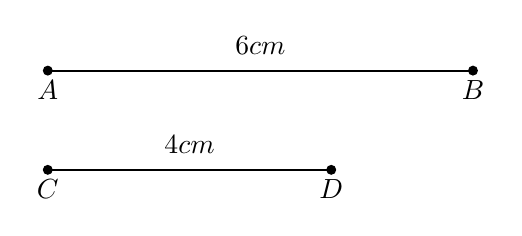
\begin{tikzpicture}[scale=0.9]

	% Segment AB
	\draw[thick] (0,0) -- (6,0);
	\fill (0,0) circle (2pt) node[below] {$A$};
	\fill (6,0) circle (2pt) node[below] {$B$};
	\node at (3,0.35) {$6\text{ cm}$};

	% Segment CD
	\draw[thick] (0,-1.4) -- (4,-1.4);
	\fill (0,-1.4) circle (2pt) node[below] {$C$};
	\fill (4,-1.4) circle (2pt) node[below] {$D$};
	\node at (2,-1.05) {$4\text{ cm}$};

\end{tikzpicture}
\caption{Comparació de dos segments. En aquest cas, \(\dfrac{AB}{CD}=\dfrac{6}{4}=\dfrac{3}{2}\).}
\label{fig:comparacio-segments}
\end{figure}

\begin{exemple}
En la figura~\ref{fig:comparacio-segments}, el segment \(\overline{AB}\) fa \(6\) cm i el segment \(\overline{CD}\) fa \(4\) cm. La raó entre les seves longituds és
\[
	\frac{AB}{CD}
	=
	\frac{6}{4}
	=
	\frac{3}{2}.
\]
Això vol dir que el segment \(\overline{AB}\) fa \(\frac{3}{2}\) vegades el segment \(\overline{CD}\).
\end{exemple}

\begin{definicio}
Direm que quatre segments \(\overline{AB}\), \(\overline{CD}\), \(\overline{EF}\) i \(\overline{GH}\) són \textbf{proporcionals} si les raons entre les seves longituds són iguals, és a dir, si
\[
	\frac{AB}{CD}
	=
	\frac{EF}{GH},
	\qquad CD\neq 0,\quad GH\neq 0.
\]
\end{definicio}

Aquesta igualtat és una proporció geomètrica. Com en qualsevol proporció, podem aplicar la propietat fonamental:
\[
	\frac{AB}{CD}
	=
	\frac{EF}{GH}
	\quad\Longleftrightarrow\quad
	AB\cdot GH=CD\cdot EF.
\]

\begin{exemple}
Suposem que
\[
	AB=8\text{ cm},\qquad CD=12\text{ cm},\qquad EF=10\text{ cm}.
\]
Volem trobar la longitud \(GH\) perquè els segments siguin proporcionals:
\[
	\frac{AB}{CD}
	=
	\frac{EF}{GH}.
\]
Substituïm les dades:
\[
	\frac{8}{12}
	=
	\frac{10}{GH}.
\]
Aplicant la propietat fonamental de les proporcions,
\[
	8\cdot GH=12\cdot 10.
\]
Per tant,
\[
	GH=\frac{120}{8}=15.
\]
Així, cal que
\[
	GH=15\text{ cm}.
\]
\end{exemple}

També podem expressar la proporcionalitat de segments mitjançant una constant de proporcionalitat. Si dos segments \(\overline{AB}\) i \(\overline{A'B'}\) compleixen
\[
	A'B'=k\cdot AB,
\]
direm que \(k\) és el \textbf{factor d'escala} que transforma el segment \(\overline{AB}\) en el segment \(\overline{A'B'}\).

Si \(k>1\), el nou segment és més llarg que l'original. Si \(0<k<1\), el nou segment és més curt. Si \(k=1\), els dos segments tenen la mateixa longitud.

\begin{exemple}
Si un segment fa \(5\) cm i l'ampliem amb factor d'escala
\[
	k=\frac{3}{2},
\]
la nova longitud serà
\[
	\frac{3}{2}\cdot 5=\frac{15}{2}=7{,}5.
\]
Per tant, el segment ampliat fa \(7{,}5\) cm.
\end{exemple}

\subsection{Segments proporcionals en figures geomètriques}

La proporcionalitat de segments és especialment important en l'estudi de figures semblants. Dues figures tenen la mateixa forma quan les longituds corresponents són proporcionals.

Per exemple, si dos triangles \(ABC\) i \(A'B'C'\) tenen costats corresponents proporcionals, podem escriure
\[
	\frac{A'B'}{AB}
	=
	\frac{B'C'}{BC}
	=
	\frac{A'C'}{AC}
	=
	k.
\]
El nombre \(k\) és el factor d'escala que transforma el triangle \(ABC\) en el triangle \(A'B'C'\).

\begin{figure}[htbp]
\centering
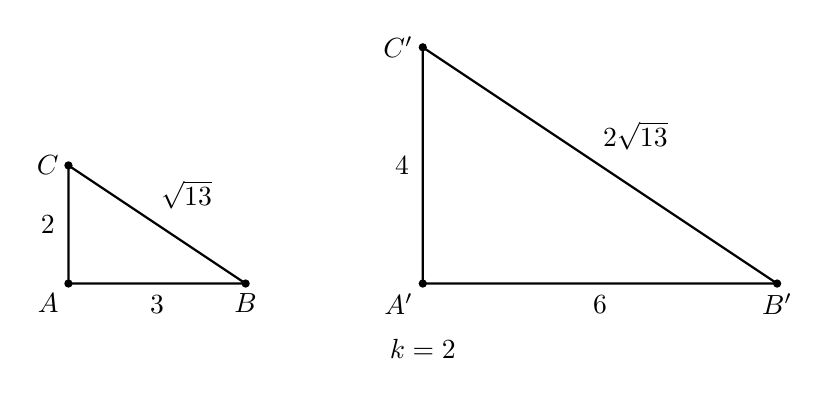
\begin{tikzpicture}[scale=0.75]

	% Primer triangle
	\coordinate (A) at (0,0);
	\coordinate (B) at (3,0);
	\coordinate (C) at (0,2);

	\draw[thick] (A) -- (B) -- (C) -- cycle;
	\fill (A) circle (2pt) node[below left] {$A$};
	\fill (B) circle (2pt) node[below] {$B$};
	\fill (C) circle (2pt) node[left] {$C$};

	\node at (1.5,-0.35) {$3$};
	\node at (-0.35,1) {$2$};
	\node at (2,1.50) {$\sqrt{13}$};

	% Segon triangle
	\coordinate (Ap) at (6,0);
	\coordinate (Bp) at (12,0);
	\coordinate (Cp) at (6,4);

	\draw[thick] (Ap) -- (Bp) -- (Cp) -- cycle;
	\fill (Ap) circle (2pt) node[below left] {$A'$};
	\fill (Bp) circle (2pt) node[below] {$B'$};
	\fill (Cp) circle (2pt) node[left] {$C'$};

	\node at (9,-0.35) {$6$};
	\node at (5.65,2) {$4$};
	\node at (9.6,2.5) {$2\sqrt{13}$};

	\node at (6,-1.1) {$k=2$};

\end{tikzpicture}
\caption{Dos triangles semblants. Les longituds del segon triangle són el doble de les longituds corresponents del primer.}
\label{fig:triangles-semblants}
\end{figure}

\begin{exemple}
En la figura~\ref{fig:triangles-semblants}, els costats corresponents dels dos triangles compleixen
\[
	\frac{A'B'}{AB}
	=
	\frac{6}{3}
	=
	2,
\]
\[
	\frac{A'C'}{AC}
	=
	\frac{4}{2}
	=
	2,
\]
i també
\[
	\frac{B'C'}{BC}
	=
	\frac{2\sqrt{13}}{\sqrt{13}}
	=
	2.
\]
Per tant, els costats corresponents són proporcionals i el segon triangle és una ampliació del primer amb factor d'escala
\[
	k=2.
\]
\end{exemple}

\subsection{El teorema de Tales}

Un dels resultats fonamentals que relaciona geometria i proporcionalitat és el teorema de Tales. Aquest teorema permet obtenir proporcions entre segments quan diverses rectes paral·leles tallen dues rectes secants.

\begin{proposicio}[Teorema de Tales]
Si diverses rectes paral·leles tallen dues rectes secants, aleshores determinen sobre aquestes rectes segments proporcionals.
\end{proposicio}

La figura~\ref{fig:tales} representa una situació típica del teorema de Tales. Les rectes verticals són paral·leles i tallen dues rectes secants que parteixen d'un mateix punt \(A\). Els segments determinats sobre una secant són proporcionals als segments corresponents determinats sobre l'altra secant.

\begin{figure}[htbp]
\centering
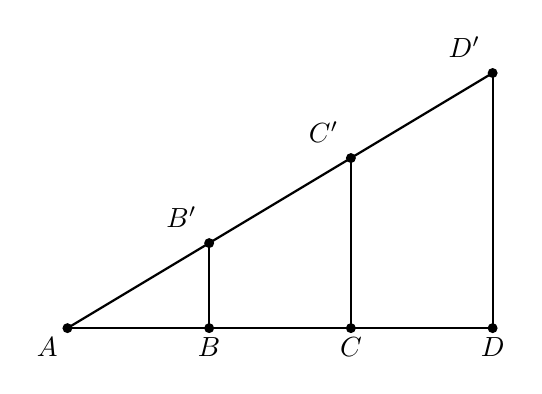
\begin{tikzpicture}[scale=0.9]

	% Punts
	\coordinate (A) at (0,0);
	\coordinate (B) at (2,0);
	\coordinate (C) at (4,0);
	\coordinate (D) at (6,0);

	\coordinate (Bp) at (2,1.2);
	\coordinate (Cp) at (4,2.4);
	\coordinate (Dp) at (6,3.6);

	% Secants
	\draw[thick] (A) -- (D);
	\draw[thick] (A) -- (Dp);

	% Paral·leles
	\draw[thick] (B) -- (Bp);
	\draw[thick] (C) -- (Cp);
	\draw[thick] (D) -- (Dp);

	% Punts i etiquetes
	\fill (A) circle (2pt) node[below left] {$A$};

	\fill (B) circle (2pt) node[below] {$B$};
	\fill (C) circle (2pt) node[below] {$C$};
	\fill (D) circle (2pt) node[below] {$D$};

	\fill (Bp) circle (2pt) node[above left,xshift=-1pt,yshift=2pt] {$B'$};
	\fill (Cp) circle (2pt) node[above left,xshift=-1pt,yshift=2pt] {$C'$};
	\fill (Dp) circle (2pt) node[above left,xshift=-1pt,yshift=2pt] {$D'$};

\end{tikzpicture}
\caption{Situació del teorema de Tales: rectes paral·leles que tallen dues rectes secants i determinen segments proporcionals.}
\label{fig:tales}
\end{figure}

En aquesta situació es compleixen proporcions com ara
\[
	\frac{AB}{BC}
	=
	\frac{AB'}{B'C'}
\]
i també
\[
	\frac{AB}{AC}
	=
	\frac{AB'}{AC'}.
\]

\begin{exemple}
Suposem que tres rectes paral·leles tallen dues rectes secants i determinen els segments següents:
\[
	AB=4\text{ cm},\qquad BC=6\text{ cm},\qquad AB'=10\text{ cm}.
\]
Volem trobar \(B'C'\). Pel teorema de Tales,
\[
	\frac{AB}{BC}
	=
	\frac{AB'}{B'C'}.
\]
Substituïm les dades:
\[
	\frac{4}{6}
	=
	\frac{10}{B'C'}.
\]
Aplicant la propietat fonamental de les proporcions,
\[
	4\cdot B'C'=6\cdot 10.
\]
Per tant,
\[
	B'C'=\frac{60}{4}=15.
\]
Així,
\[
	B'C'=15\text{ cm}.
\]
\end{exemple}

\subsection{Escales, ampliacions i reduccions}

Una aplicació directa de la proporcionalitat geomètrica és l'ús d'escales en mapes, plànols i maquetes.

Una escala indica la raó entre una longitud representada i la longitud real corresponent. Per exemple, una escala
\[
	1:100
\]
vol dir que \(1\) unitat en el dibuix representa \(100\) unitats en la realitat.

Si la longitud en el dibuix és \(d\) i la longitud real és \(r\), aleshores
\[
	\frac{d}{r}
	=
	\frac{1}{100}.
\]

\begin{exemple}
En un plànol a escala \(1:200\), una habitació fa \(4\) cm de llarg. Quina és la longitud real de l'habitació?

L'escala \(1:200\) vol dir que
\[
	1\text{ cm en el plànol}=200\text{ cm en la realitat}.
\]
Per tant,
\[
	4\text{ cm en el plànol}=4\cdot 200=800\text{ cm en la realitat}.
\]
Com que
\[
	800\text{ cm}=8\text{ m},
\]
la longitud real de l'habitació és
\[
	8\text{ m}.
\]
\end{exemple}

\begin{exemple}
Una maqueta està feta a escala \(1:50\). Si una paret real fa \(12\) m, quina longitud tindrà en la maqueta?

Primer expressem la longitud real en centímetres:
\[
	12\text{ m}=1200\text{ cm}.
\]
Com que l'escala és \(1:50\), la longitud en la maqueta serà
\[
	\frac{1200}{50}=24.
\]
Per tant, la paret farà
\[
	24\text{ cm}
\]
en la maqueta.
\end{exemple}

\subsection{Observació sobre les raons geomètriques}

En aquesta unitat treballem principalment amb raons racionals, perquè l'objectiu és estudiar els nombres racionals i les seves aplicacions. Ara bé, en geometria també apareixen raons que no són racionals.

Per exemple, en un quadrat de costat \(1\), la diagonal té longitud \(\sqrt{2}\). La raó entre la diagonal i el costat és
\[
	\frac{\sqrt{2}}{1}
	=
	\sqrt{2},
\]
que no és un nombre racional.

Això mostra que la geometria porta de manera natural més enllà dels nombres racionals. Aquest fet serà important quan s'estudiïn els nombres irracionals i, posteriorment, els nombres reals.


\section{Funcions de proporcionalitat}

A la secció anterior hem estudiat la proporcionalitat directa i la proporcionalitat inversa com a relacions entre magnituds. Ara les reinterpretarem com a funcions, és a dir, com a correspondències que assignen a cada valor admissible d'una variable \(x\) un únic valor d'una variable \(y\).

Tot i que en aquesta unitat treballem amb nombres racionals, per visualitzar aquestes funcions en el pla cartesià dibuixarem la recta o la corba corresponent. Els punts amb coordenades racionals en formen part.

\subsection{Funció de proporcionalitat directa}

Una funció de proporcionalitat directa és una funció de la forma
\[
	f(x)=kx,
\]
on \(k\in\Q\) és una constant.

La seva gràfica és una recta que passa per l'origen de coordenades.

\begin{exemple}
Considerem la funció
\[
	f(x)=2x.
\]
Aquesta és una funció de proporcionalitat directa amb constant de proporcionalitat \(k=2\).
\end{exemple}

\begin{solucio}
Calculem alguns valors:
\[
\begin{array}{c|ccccc}
x & -2 & -1 & 0 & 1 & 2 \\
\hline
f(x)=2x & -4 & -2 & 0 & 2 & 4
\end{array}
\]

Representem ara alguns punts de coordenades racionals que satisfan la relació
\[
	y=2x.
\]
Observem que tots aquests punts queden alineats. Si treballéssim sobre \(\R\), la seva representació gràfica seria una recta que passa per l'origen.

\begin{center}
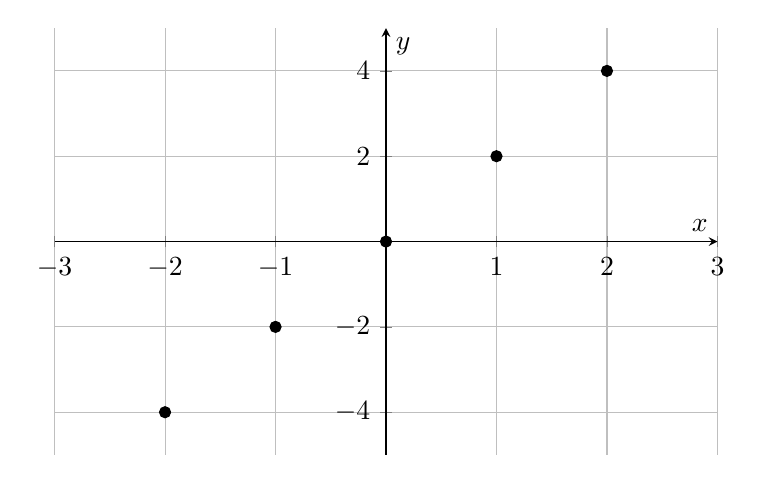
\begin{tikzpicture}
\begin{axis}[
	axis lines=middle,
	xlabel={$x$},
	ylabel={$y$},
	xmin=-3, xmax=3,
	ymin=-5, ymax=5,
	grid=both,
	width=10cm,
	height=7cm
]
\addplot[
	only marks,
	mark=*,
	black
]
coordinates {
	(-2,-4)
	(-1,-2)
	(0,0)
	(1,2)
	(2,4)
};
\end{axis}
\end{tikzpicture}

\smallskip
\textit{Punts de la funció de proporcionalitat directa \(f(x)=2x\).}
\end{center}

Així, la funció \(f(x)=2x\) és una recta que passa per l'origen. Això és característic de totes les funcions de proporcionalitat directa.
\end{solucio}

\subsection{Funció de proporcionalitat inversa}

Una funció de proporcionalitat inversa és una funció de la forma
\[
	f(x)=\frac{k}{x},
\]
on \(k\in\Q\), \(k\neq0\), és una constant.

Aquesta funció no està definida en \(x=0\), i la seva gràfica és una hipèrbola.

\begin{exemple}
Considerem la funció
\[
	f(x)=\frac{6}{x}.
\]
Aquesta és una funció de proporcionalitat inversa amb constant de proporcionalitat \(k=6\).
\end{exemple}

\begin{solucio}
Calculem alguns valors:
\[
\begin{array}{c|cccccccc}
x & -6 & -3 & -2 & -1 & 1 & 2 & 3 & 6 \\
\hline
f(x)=\frac{6}{x} & -1 & -2 & -3 & -6 & 6 & 3 & 2 & 1
\end{array}
\]

Representem ara alguns punts de coordenades racionals que satisfan la relació
\[
	y=\frac{6}{x}.
\]
Observem que aquests punts no estan alineats i es distribueixen en dues branques. Si treballéssim sobre \(\R\), la seva representació gràfica seria una hipèrbola.

\begin{center}
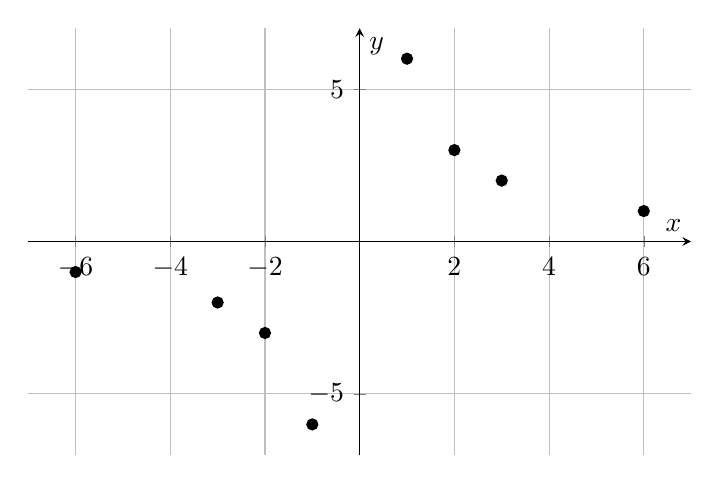
\begin{tikzpicture}
\begin{axis}[
	axis lines=middle,
	xlabel={$x$},
	ylabel={$y$},
	xmin=-7, xmax=7,
	ymin=-7, ymax=7,
	grid=both,
	width=10cm,
	height=7cm
]
\addplot[
	only marks,
	mark=*,
	black
]
coordinates {
	(-6,-1)
	(-3,-2)
	(-2,-3)
	(-1,-6)
	(1,6)
	(2,3)
	(3,2)
	(6,1)
};
\end{axis}
\end{tikzpicture}

\smallskip
\textit{Punts de la funció de proporcionalitat inversa \(f(x)=\frac{6}{x}\).}
\end{center}
\end{solucio}

\begin{observacio}
Les funcions de proporcionalitat directa i inversa es poden distingir fàcilment per la seva expressió algebraica i per la seva gràfica:
\begin{itemize}
	\item si
	\[
		f(x)=kx,
	\]
	la gràfica és una recta que passa per l'origen;
	\item si
	\[
		f(x)=\frac{k}{x},
	\]
	la gràfica és una hipèrbola i la funció no està definida en \(x=0\).
\end{itemize}
\end{observacio}

\subsection{Comparació entre proporcionalitat directa i inversa}

La diferència essencial entre els dos tipus de proporcionalitat és la magnitud que es manté constant.

En una proporcionalitat directa, el quocient és constant:
\[
	\frac{y}{x}=k.
\]
Per això la relació es pot escriure com
\[
	y=kx.
\]

En una proporcionalitat inversa, el producte és constant:
\[
	xy=k.
\]
Per això la relació es pot escriure com
\[
	y=\frac{k}{x}.
\]

\[
\begin{array}{c|c|c}
\text{Tipus de proporcionalitat} & \text{Relació constant} & \text{Funció associada}\\
\hline
\text{Directa} & \dfrac{y}{x}=k & y=kx\\[1.2em]
\text{Inversa} & xy=k & y=\dfrac{k}{x}
\end{array}
\]

Aquesta distinció és important perquè moltes situacions es resolen de manera diferent segons si les magnituds són directament proporcionals o inversament proporcionals. Abans d'aplicar una regla de tres, cal determinar quin tipus de proporcionalitat hi ha. 